%%% The main file. It contains definitions of basic parameters and includes all other parts.

% Meta-data of your thesis (please edit)
\input metadata.tex

% Generate metadata in XMP format for use by the pdfx package
\input xmp.tex

%% Settings for single-side (simplex) printing
% Margins: left 40mm, right 25mm, top and bottom 25mm
% (but beware, LaTeX adds 1in implicitly)
\documentclass[12pt,a4paper]{report}
\setlength\textwidth{145mm}
\setlength\textheight{247mm}
\setlength\oddsidemargin{15mm}
\setlength\evensidemargin{15mm}
\setlength\topmargin{0mm}
\setlength\headsep{0mm}
\setlength\headheight{0mm}
% \openright makes the following text appear on a right-hand page
\let\openright=\clearpage

%% Settings for two-sided (duplex) printing
% \documentclass[12pt,a4paper,twoside,openright]{report}
% \setlength\textwidth{145mm}
% \setlength\textheight{247mm}
% \setlength\oddsidemargin{14.2mm}
% \setlength\evensidemargin{0mm}
% \setlength\topmargin{0mm}
% \setlength\headsep{0mm}
% \setlength\headheight{0mm}
% \let\openright=\cleardoublepage

%% If the thesis has no printed version, symmetric margins look better
% \documentclass[12pt,a4paper]{report}
% \setlength\textwidth{145mm}
% \setlength\textheight{247mm}
% \setlength\oddsidemargin{10mm}
% \setlength\evensidemargin{10mm}
% \setlength\topmargin{0mm}
% \setlength\headsep{0mm}
% \setlength\headheight{0mm}
% \let\openright=\clearpage

%% Generate PDF/A-2u
\usepackage[a-2u]{pdfx}

%% Prefer Latin Modern fonts
\usepackage{lmodern}
% If we are not using LuaTeX, we need to set up character encoding:
\usepackage{iftex}
\ifpdftex
\usepackage[utf8]{inputenc}
\usepackage[T1]{fontenc}
\usepackage{textcomp}
\fi

%% Further useful packages (included in most LaTeX distributions)
\usepackage{amsmath}        % extensions for typesetting of math
\usepackage{amsfonts}       % math fonts
\usepackage{amsthm}         % theorems, definitions, etc.
\usepackage{bm}             % boldface symbols (\bm)
\usepackage{booktabs}       % improved horizontal lines in tables
\usepackage{caption}        % custom captions of floating objects
\usepackage{dcolumn}        % improved alignment of table columns
\usepackage{floatrow}       % custom float environments
\usepackage{graphicx}       % embedding of pictures
\usepackage{indentfirst}    % indent the first paragraph of a chapter
\usepackage[nopatch=item]{microtype}   % micro-typographic refinement
\usepackage{paralist}       % improved enumerate and itemize
\usepackage[nottoc]{tocbibind} % makes sure that bibliography and the lists
			    % of figures/tables are included in the table
			    % of contents
\usepackage{xcolor}         % typesetting in color

% The hyperref package for clickable links in PDF and also for storing
% metadata to PDF (including the table of contents).
% Most settings are pre-set by the pdfx package.
\hypersetup{unicode}
\hypersetup{breaklinks=true}

% Packages for computer science theses
% https://tex.stackexchange.com/questions/145760/how-may-i-remove-endif-and-endfor-in-algorithmicx/145764#145764
%\usepackage{algpseudocode}  % part of algorithmicx package
\usepackage[noend]{algpseudocode}  % use noend to not display endif, endfor, etc.

% https://latex.org/forum/viewtopic.php?t=15388
%\usepackage{algorithm}
\usepackage[plain]{algorithm} % use plain to remove horizontal lines in algorithm

\usepackage{fancyvrb}       % improved verbatim environment
\usepackage{listings}       % pretty-printer of source code

% You might want to use cleveref for references
% \usepackage{cleveref}

% Set up formatting of bibliography (references to literature)
% Details can be adjusted in macros.tex.
%
% BEWARE: Different fields of research and different university departments
% have their own customs regarding bibliography. Consult the bibliography
% format with your supervisor.
%
% The basic format according to the ISO 690 standard with numbered references
\usepackage[natbib,style=iso-numeric,sorting=none]{biblatex}
% ISO 690 with alphanumeric references (abbreviations of authors' names)
%\usepackage[natbib,style=iso-alphabetic]{biblatex}
% ISO 690 with references Author (year)
%\usepackage[natbib,style=iso-authoryear]{biblatex}
%
% Some fields of research prefer a simple format with numbered references
% (sorting=none tells that bibliography should be listed in citation order)
%\usepackage[natbib,style=numeric,sorting=none]{biblatex}
% Numbered references, but [1,2,3,4,5] is compressed to [1-5]
%\usepackage[natbib,style=numeric-comp,sorting=none]{biblatex}
% A simple format with alphanumeric references:
%\usepackage[natbib,style=alphabetic]{biblatex}

% Load the file with bibliography entries
\addbibresource{bibliography.bib}

% Our definitions of macros (see description inside)
\input macros.tex

% Include automatic generation of abbreviations
% \usepackage{glossaries-extra}
% \makeglossaries
% \input abbreviations.tex

%%% Title page and various mandatory informational pages
\begin{document}
%%% Title page of the thesis and other mandatory pages

%%% Inscriptions at the opening page of the hard cover

% We usually do not typeset the hard cover, but if you want to do it, change \iffalse to \iftrue
\iffalse

\pagestyle{empty}
\hypersetup{pageanchor=false}
\begin{center}

\large
Charles University

\medskip

Faculty of Mathematics and Physics

\vfill

{\huge\bf\ThesisTypeTitle}

\vfill

{\huge\bf\ThesisTitle\par}

\vfill
\vfill

\hbox to \hsize{\YearSubmitted\hfil \ThesisAuthor}

\end{center}

\newpage\openright
\setcounter{page}{1}

\fi

%%% Title page of the thesis

\pagestyle{empty}
\hypersetup{pageanchor=false}
\begin{center}

\centerline{\mbox{
\includegraphics[width=166mm]{img/logo-en.pdf}}}

\vspace{-8mm}
\vfill

{\bf\Large\ThesisTypeTitle}

\vfill

{\LARGE\ThesisAuthor}

\vspace{15mm}

{\LARGE\bfseries\ThesisTitle\par}

\vfill

\Department

\vfill

{
\centerline{\vbox{\halign{\hbox to 0.45\hsize{\hfil #}&\hskip 0.5em\parbox[t]{0.45\hsize}{\raggedright #}\cr
Supervisor of the \ThesisTypeName{} thesis:&\Supervisor \cr
\ifx\ThesisType\TypeRig\else
\noalign{\vspace{2mm}}
Study programme:&\StudyProgramme \cr
\fi
}}}}

\vfill

Prague \YearSubmitted

\end{center}

\newpage

%%% A page with a solemn declaration to the thesis

\openright
\hypersetup{pageanchor=true}
\vglue 0pt plus 1fill

\noindent
I declare that I carried out this \ThesisTypeName{} thesis on my own, and only with the cited
sources, literature and other professional sources.
I understand that my work relates to the rights and obligations under the Act No.~121/2000 Sb.,
the Copyright Act, as amended, in particular the fact that the Charles
University has the right to conclude a license agreement on the use of this
work as a school work pursuant to Section 60 subsection 1 of the Copyright~Act.

\vspace{10mm}

\hbox{\hbox to 0.5\hsize{%
In \hbox to 6em{\dotfill} date \hbox to 6em{\dotfill}
\hss}\hbox to 0.5\hsize{\dotfill\quad}}
\smallskip
\hbox{\hbox to 0.5\hsize{}\hbox to 0.5\hsize{\hfil Author's signature\hfil}}

\vspace{20mm}
\newpage

%%% Dedication

\openright

\noindent
\Dedication

\newpage

%%% Mandatory information page of the thesis

\openright
{\InfoPageFont

\vtop to 0.5\vsize{
\setlength\parindent{0mm}
\setlength\parskip{5mm}

Title:
\ThesisTitle

Author:
\ThesisAuthor

\DeptType:
\Department

Supervisor:
\Supervisor, \SupervisorsDepartment

Abstract:
\Abstract

Keywords:
{\def\sep{\unskip, }\ThesisKeywords}

\vfil
}

% In Czech study programmes, it is mandatory to include Czech meta-data:

\ifx\StudyLanguage\LangCS

\vtop to 0.49\vsize{
\setlength\parindent{0mm}
\setlength\parskip{5mm}

Název práce:
\ThesisTitleCS

Autor:
\ThesisAuthor

\DeptTypeCS:
\DepartmentCS

Vedoucí bakalářské práce:
\Supervisor, \SupervisorsDepartmentCS

Abstrakt:
\AbstractCS

Klíčová slova:
{\def\sep{\unskip, }\ThesisKeywordsCS}

\vfil
}

\fi

}

\newpage

%%% Further pages will be numbered
\pagestyle{plain}


%%% A page with automatically generated table of contents of the thesis

\tableofcontents

%%% Each chapter is kept in a separate file
\chapter*{Introduction}
\addcontentsline{toc}{chapter}{Introduction}

%Zadání
%
%Simulace problému z Google Hash Code 2021 a jeho optimalizace pomocí různých technik umělé inteligence Genetický algoritmus, Local search, Simulated annealing a porovnání těchto přístupů
%
%Cílem je efektivně implementovat simulaci a vyzkoušet různé algoritmy pro její optimalizaci, nikoliv implementovat samotné optimalizační algoritmy (avšak pokud bude vhodnější genetické algoritmy/local search ručně naimplementovat než použít knihovnu, bude to možné, ale není to cílem)
%
%
% Zásady pro vypracování
% Student se ve své práci bude věnovat řízení množiny křižovatek zadané grafem dle specifikace Google Hash Code [1].
% Student práci začne implementací vlastního simulátoru křižovatek dle uvedené specifikace, který bude používat k optimalizaci řízení.
% K optimalizaci student s použitím vhodných nástrojů implementuje a následně experimentálně porovná následující algoritmy.
% 1) Evoluční algoritmy
% 2) Lokální prohledávání
% Na základě získaných zkušeností student dále zvolí některý z následujících přístupů.
% 3) Memetiské algoritmy
% 4) Metaheuristiky
% 5) Náhradní modely

Due to its significant impact on urban mobility and the environment, Traffic Signal Control (TSC) is a widely studied problem. As the number of vehicles on the road continues to increase, its importance is growing even further.
Traffic Signal Optimization is known to be a cost-effective method for reducing congestion without physically changing the road infrastructure.
Optimized traffic lights reduce delays at intersections, which directly translates into time savings for commuters and improves the overall efficiency of transportation networks.
Additionally, TSC plays a critical role in reducing vehicle emissions, helping to reduce pollution and promote environmental sustainability.

There are many approaches \cite{qadri2020state} to solving TSC. Early static, fixed-time designs have evolved into real-time adaptive systems and data-driven algorithms, utilizing data from various detectors and sensors. In practice, commonly used are adaptive traffic control systems (ATCS) such as SCOOT, SCATS, and SURTRAC \cite{smith2013surtrac}, which continuously adjust splits, offsets, and cycle lengths network-wide. In addition, optimization-based methods---such as genetic algorithms, metaheuristics, and Model Predictive Control (MPC)---have also been employed for traffic signal planning and coordination \cite{qadri2020state, ye2019survey}. More recently, learning-based methods, particularly those based on Reinforcement Learning (RL) and Deep Reinforcement Learning (DRL), have demonstrated superior performance compared to traditionally used methods \cite{zhao2024survey, saadi2025survey}.

\section*{Contribution of the thesis}

\xxx{Blackbox optimization}

In this thesis, we focus on the Traffic signaling problem from the Google Hash Code 2021 competition. It serves as a simplified version of the real-world problem of traffic light optimization in a city. First, we implement a fast and efficient C++ simulator of the problem and wrap it as a Python package to allow for easy use and integration with the wide ecosystem of Python libraries. Then, we use the simulator to optimize the traffic light schedules using three heuristic algorithms: Genetic Algorithm (GA), Hill Climbing (HC), and Simulated Annealing (SA). We experimentally compare the performance of these algorithms on provided datasets of different sizes and structures.

The thesis is structured as follows. Chapter~\ref{chap:problem_description} describes the Traffic signaling problem in detail, including the city layout, cars, traffic lights, and scoring system. Chapter~\ref{chap:optimization_methods} covers the theory of the optimization algorithms used in this thesis. Chapter ...

Chapter~\ref{chap:experiments} presents the expertiments comparing the optimization algorithms on the provided datasets.

\xxx{Unused citations: Principled Modeling of the Google Hash Code Problems for Meta-Heuristics \cite{rodrigues2023principled}, Building a Simulator and Emulator for Traffic Signaling \cite{li2022building}.}

\chapter{Problem description} \label{chap:problem_description}

This chapter introduces the optimization problem addressed in this thesis. Section~\ref{sec:competition_overview} provides a brief overview of the competition setting where the problem was initially assigned. In Section~\ref{sec:original_problem_statement}, the original problem statement is presented and explained in detail.
Section~\ref{sec:preprocessing} explains preprocessing steps that we apply to simplify the problem for optimization.
Section~\ref{sec:datasets} describes the datasets provided with the problem. Finally, Section~\ref{sec:simulator} presents the custom simulator tool that we developed to evaluate solutions to the problem.

\section{Competition overview} \label{sec:competition_overview}

The problem we address in this thesis was originally assigned in the qualifying round of Google Hash Code 2021. Google Hash Code was a global team programming competition, running between 2014--2022, where teams of 2--4 competitors solved an optimization problem with the goal of achieving the best score in a limited time of 4 hours. Despite its discontinuation, the competition remains a valuable resource for a wide range of optimization problems and have been the subject of various follow-up studies and articles~\cite{rodrigues2023principled, li2022building}.

The usual solution procedure for our problem was as follows: Read the input data, create a trivial solution and write it to the output file in the specified format, and upload the solution to the evaluation system. The evaluation system not only displayed the score, but also some informative statistics, such as the number of cars that reached the finish before the deadline, the cars that arrived earliest and latest, the average cycle length of traffic lights at intersections, etc.
For some datasets, an interactive visualization of the evaluation process was also available, allowing to see the structure of a particular dataset. Although a local simulator was not needed to solve the problem, the manual upload of the solution to the evaluation system was slow and cumbersome and therefore not suitable for the use of efficient optimization algorithms.

Most teams were able to construct trivial solutions, which they then tried to improve by randomly changing the values. However, the best teams were able to write their own local simulator and use it to run multiple heuristics to get a better total score. Still, there was no time for anything more complex than a simple random search.

The total score was the sum of the scores of all 6 datasets (A--F). The first dataset (A) served as a ``toy problem'' mainly for debugging purposes, but the rest of the datasets were large enough for optimization. It should be noted that the distribution of points among the datasets is uneven, so the contestants mostly focused on the datasets with the highest possible score (D, F) and pragmatically skipped optimizing the rest (B, C, E).

\section{Original problem statement} \label{sec:original_problem_statement}

The full problem statement\footnote{\url{https://github.com/google/coding-competitions-archive/blob/main/hashcode/hashcode_2021_qualification_round.pdf}} is available in the Google Coding Competitions archive~\cite{google2023google}. Here we describe only the parts that are important for understanding this work.
In short, the task is as follows:
\begin{quote}
    \textit{Given a city plan describing intersections and streets and cars with planned paths through the city, optimize the schedule of traffic lights to minimize the total amount of time spent in traffic, and help as many cars as possible reach their destination before a specified deadline.}
\end{quote}
In terms of graph theory, the city plan is a \textit{directed graph}. The intersections are \textit{vertices} and the streets are \textit{directed edges} (see Figure~\ref{fig:hashcode_city_plan}). The planned path for each car is indeed a \textit{path} in this graph because it has a different start and end, and no intersection is repeated.

\begin{figure}
    \centering
    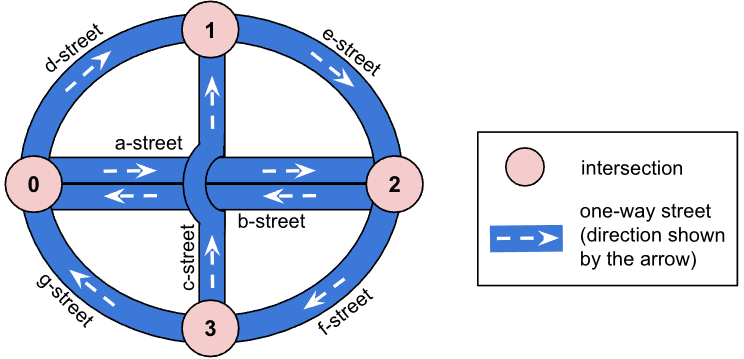
\includegraphics[width=\linewidth]{img/hashcode/figure1.png}
    %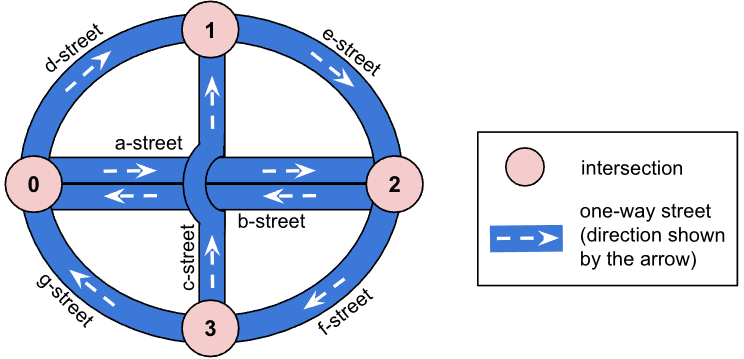
\includegraphics[width=.8\linewidth]{img/hashcode/figure1.png}
    \caption[Example of a city plan]{
        Example of a city plan \cite{google2023google}.
    }
    \label{fig:hashcode_city_plan}
\end{figure}

\subsection{Streets and intersections}

In the city, we have a set of intersections
$I$, where $\abs{I} \in [2, 10^5]$,
and a set of streets
$S \subseteq \{(u, v) | u,v \in I \land u \neq v\}$, where $\abs{S} \in [2, 10^5]$.
Each street $s \in S$ is a unique one-way connection between two different intersections $u$, $v$; two distinct streets $(u, v)$ and $(v, u)$ in opposite directions between the same two intersections are allowed. Each street $s \in S$ has a fixed time $l(s) \in \mathbb{N}_+$ that it takes a car to get from the beginning to the end of the street, independently of the other cars on the street.
Each intersection $i \in I$ has a set of incoming streets $S_i^+ \subset S$, where $\abs{S_i^+} \geq 1$, and a set of outgoing streets $S_i^- \subset S$, where $\abs{S_i^-} \geq 1$; thus each intersection has at least one incoming street and at least one outgoing street.

\subsection{Traffic lights and schedules}

In each intersection $i \in I$, there is a traffic light at the end of each \textit{incoming} street $s^+ \in S_i^+$. The traffic light has two states---green and red. Green means the cars from this street can pass through the intersection and continue to any \textit{outgoing} street $s^- \in S_i^-$ in their path. Red means the cars must stop until the light turns green again. At most one traffic light can be green at each intersection at any time.

When the light is red, cars arriving at the end of a street queue up and wait for the light to turn green. The queue does not take up any space and does not change the distance cars have to travel. When the light is green, one car can pass through an intersection every second. Passing through an intersection, i.e., moving from the end of an incoming street to the beginning of an outgoing street, takes no additional time.

For each intersection $i \in I$, we can set a traffic light schedule. This schedule determines the order and duration of green light for the incoming streets of the intersection. The schedule repeats in a cycle until the end of the simulation (see Figure~\ref{fig:hashcode_traffic_lights}). Each street can appear at most once in the schedule. If a street is not included in the schedule, it is red the whole time, and any waiting cars are blocked. By default, intersections have no schedule and all streets are red.

% https://tex.stackexchange.com/questions/69869/image-taking-up-full-page
\begin{figure}[ht] % h = here, t = top, p = page of floats
    \centering
    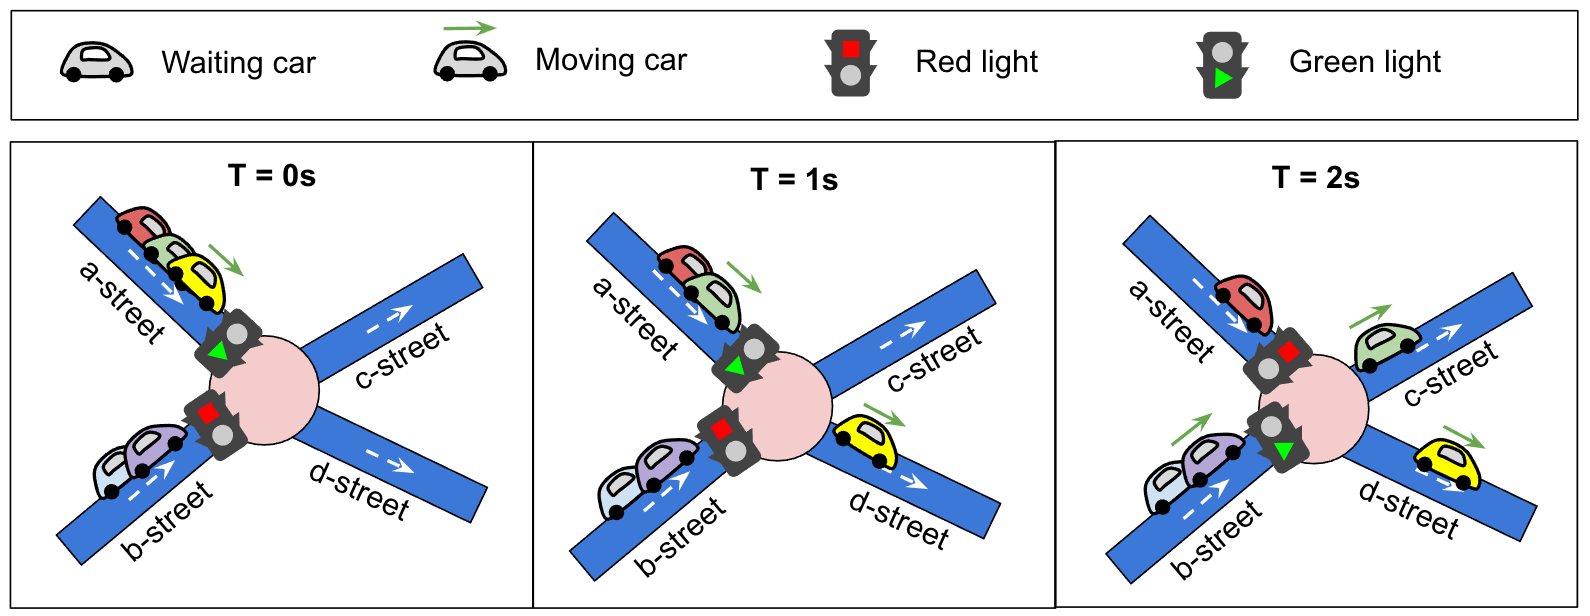
\includegraphics[width=\linewidth]{img/hashcode/figure2-abc.png}
    % 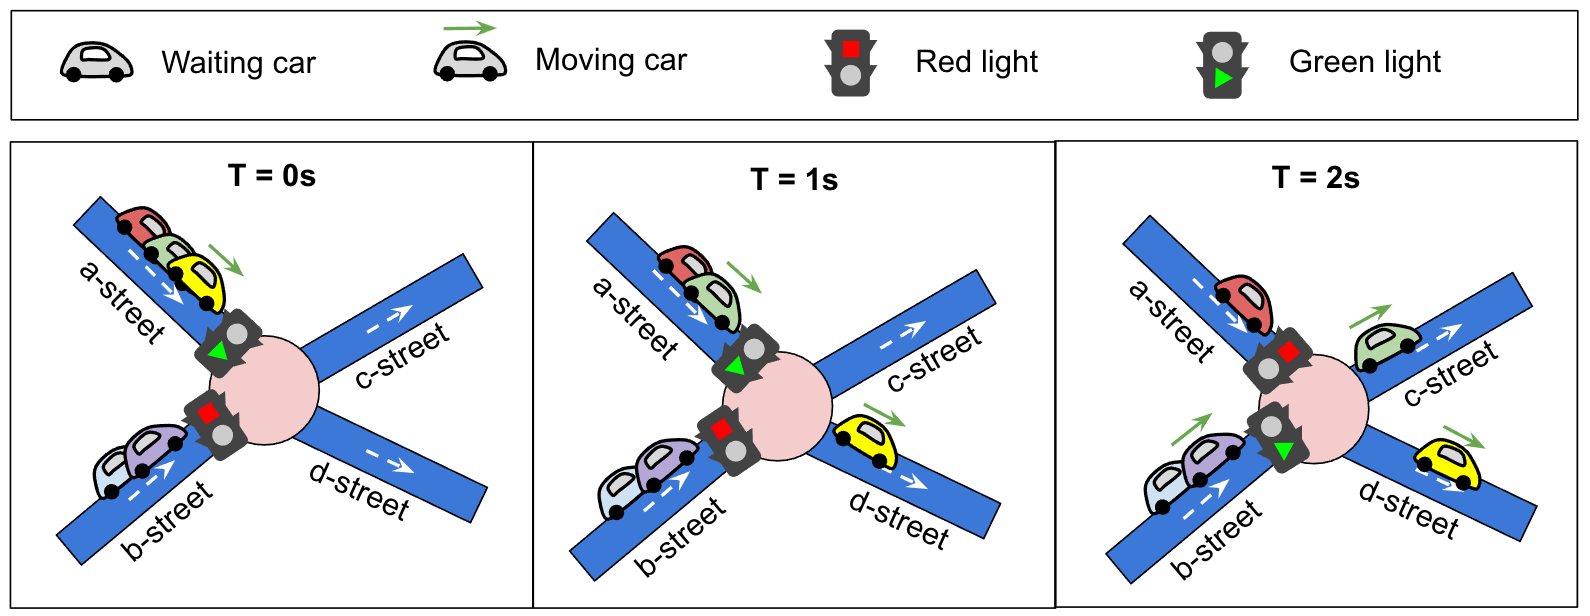
\includegraphics[width=.8\linewidth]{img/hashcode/figure2-abc.png}
    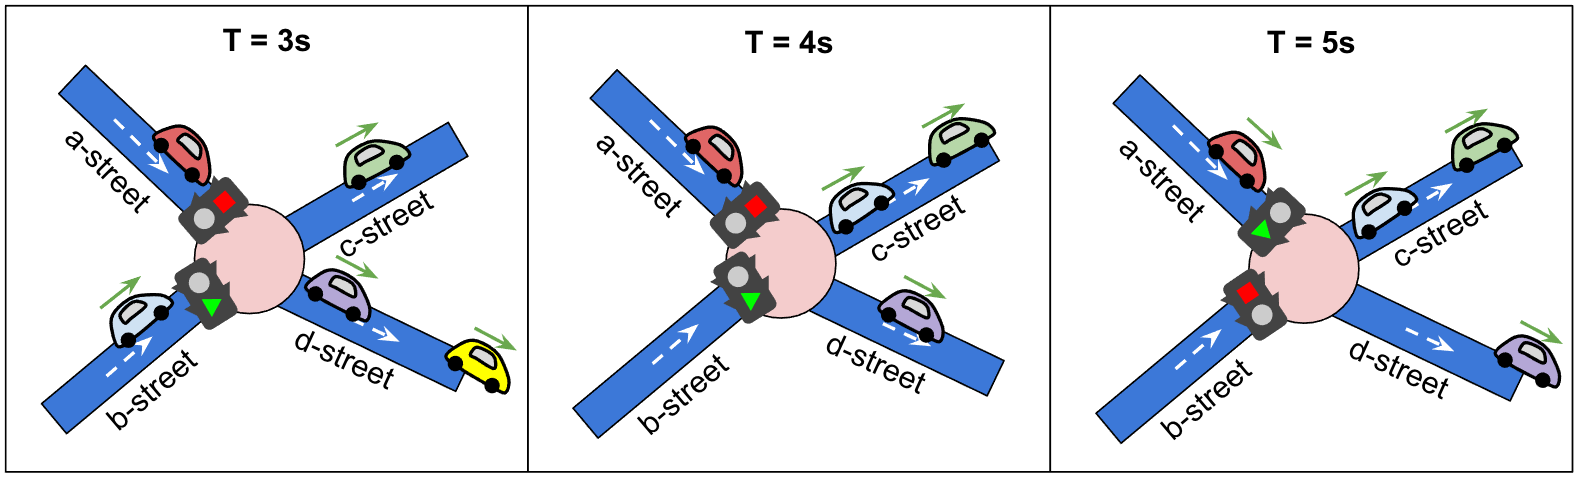
\includegraphics[width=\linewidth]{img/hashcode/figure2-def.png}
    % 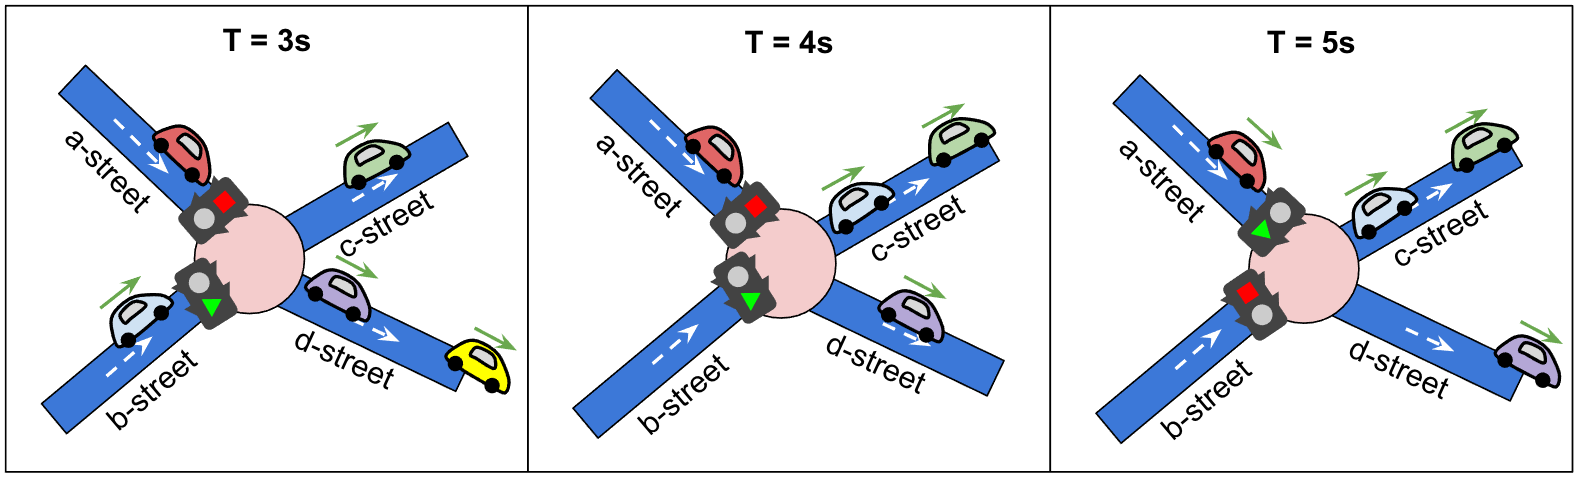
\includegraphics[width=.8\linewidth]{img/hashcode/figure2-def.png}
    \caption[Example of a traffic light schedule]{
        This figure shows how the traffic light schedule works for an intersection with two incoming streets \cite{google2023google}.
        The schedule is as follows: First \textit{a-street} for $2$ seconds, then \textit{b-street} for $3$ seconds.
        We can see the first two cars from \textit{a-street} pass in the first two seconds, then the green light switches to \textit{b-street} for three seconds,
        allowing the two cars from \textit{b-street} pass. The last car from \textit{a-street} waits till the beginning of the next cycle and then passes.
    }
    \label{fig:hashcode_traffic_lights}
\end{figure}

\subsection{Cars}

Furthermore, we have a set of cars $C$, where $\abs{C} \in [1, 10^3]$. Each car $c \in C$ has a given path $\bm{p_c}$ through the city. The path is a sequence of streets the car has to drive through.
The number of streets in each path $\bm{p_c}$ is in the range $[2, 10^3]$.
No intersection or street can be repeated in a path.

At the beginning of the simulation, all cars are at the end of the first street in their path. They either wait if the light is red or are ready to move if the light is green. If more cars start at the end of the same street, they queue up according to their IDs in the input file (see Figure~\ref{fig:hashcode_street}). When a car reaches the end of the last street in its path, it is immediately removed from the street.

\begin{figure}[ht] % h = here, t = top, p = page of floats
    \centering
    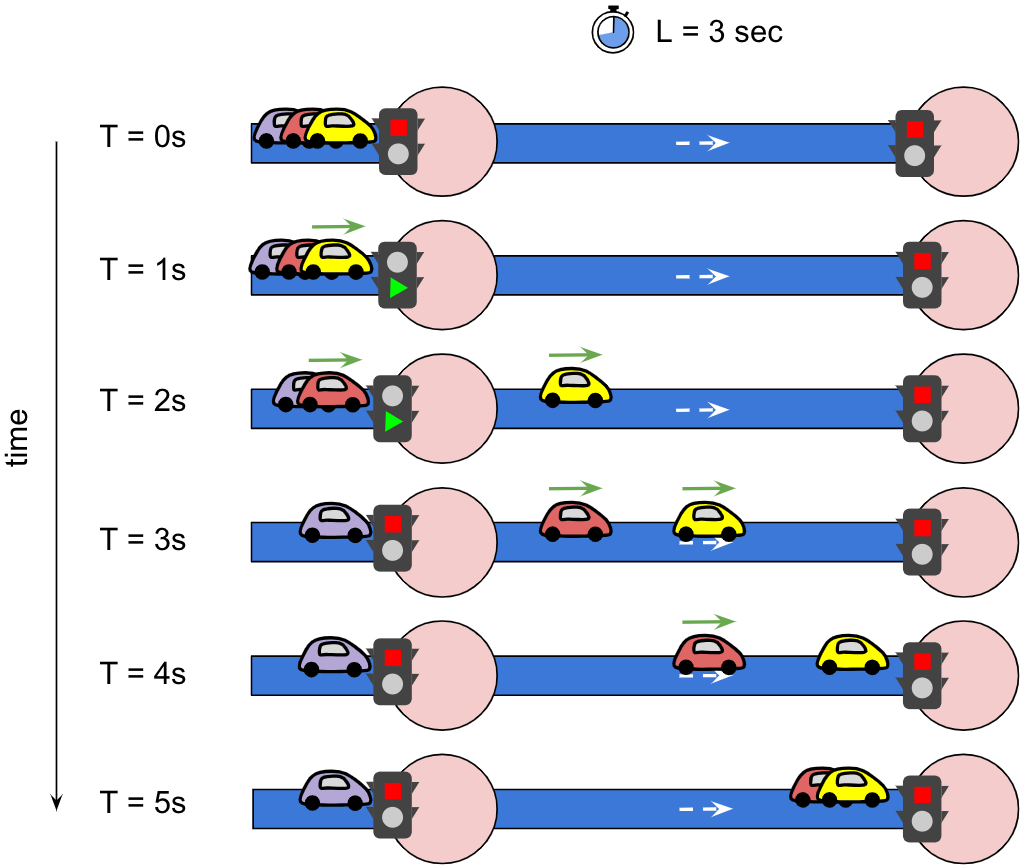
\includegraphics[width=\linewidth]{img/hashcode/figure3.png}
    %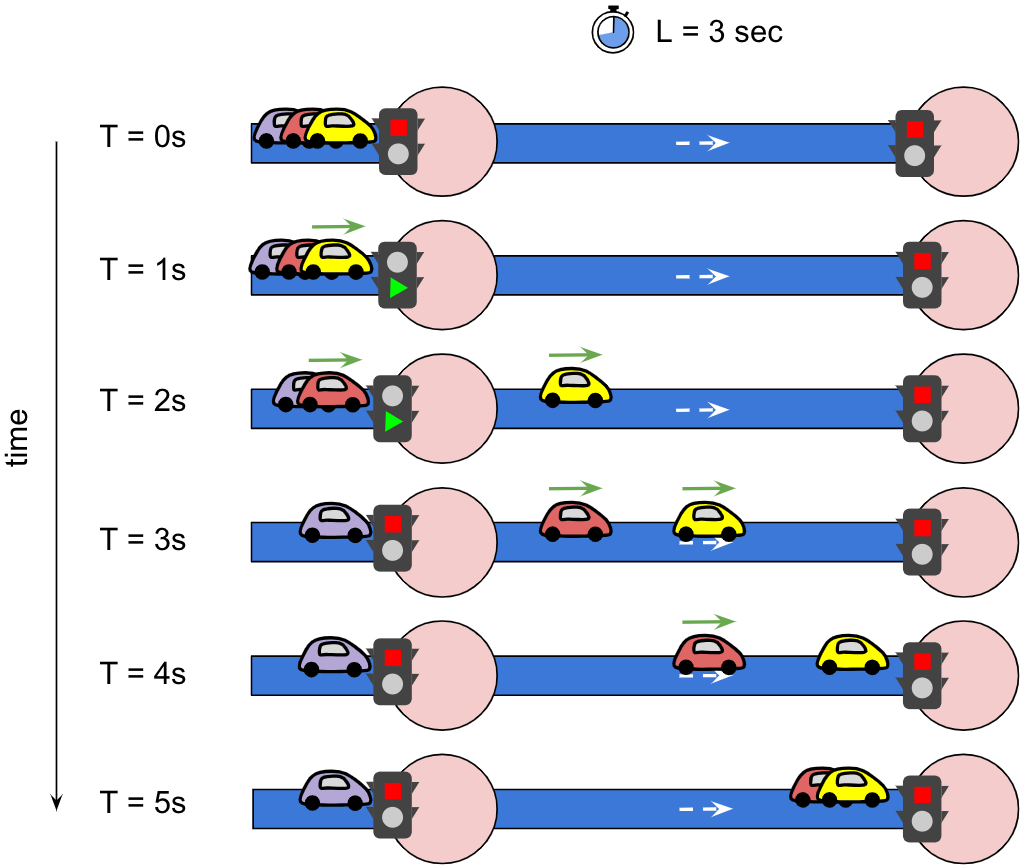
\includegraphics[width=.8\linewidth]{img/hashcode/figure3.png}
    \caption[Example of cars driving through a street]{
        This figure shows the first five seconds of a~simulation \cite{google2023google}.
        For simplicity, only one street is shown in the figure; when the light is red for this street, it is green for another street in the same intersection.
        When the light turns green at $T=1s$, the first (yellow) car immediately passes the intersection and moves to the next street, reaching the end of the street at $T=4s$.
        At $T=2s$, the light is still green, so the second (red) car passes the intersection and moves to the next street, reaching the end of the street at $T=5s$.
        From $T=3s$ to $T=5s$, the light is red, so the third (purple) car cannot pass the intersection and has to wait for the next cycle.
    }
    \label{fig:hashcode_street}
\end{figure}

\subsection{Score}

The score reflects the quality of the traffic light schedules: the more cars reach their destination, and the sooner they arrive, the higher the score.
The objective is to maximize this value.
In the context of optimization, the score serves as a \textit{fitness function}.

The score is determined as follows. Let $\bm{\theta}$ denote the traffic light schedules, and let $C$ be the set of cars.
Given a simulation duration $\mathrm{D} \in [1, 10^4]$ in seconds,
and a fixed bonus awarded for reaching the destination $\mathrm{F} \in [1, 10^3]$,
let $t(c; \bm{\theta}) \in \mathbb{N}$ be the time when a car $c \in C$ reaches its destination.
The score of a single car $c$ under the schedules $\bm{\theta}$ is defined as
\begin{equation}
    score(c; \bm{\theta}) =
    \begin{cases}
        \mathrm{F} + (\mathrm{D} - t(c; \bm{\theta})), & \text{if $t(c; \bm{\theta}) \leq \mathrm{D}$}, \\
        0, & \text{otherwise}.
    \end{cases}
\end{equation}
Then, the total score of the schedules $\bm{\theta}$ is defined as
\begin{equation}
    SCORE(\bm{\theta}) = \sum_{c \in C} score(c; \bm{\theta}).
\end{equation}

\section{Preprocessing of a problem instance} \label{sec:preprocessing}

In this section, we introduce preprocessing steps that we apply to reduce the total number of parameters we need to optimize.
These are our own observations and are not part of the original problem statement. After preprocessing, a substantial amount of intersections and streets is removed from optimization, which allows us to save resources and focus only on the important parameters. We also describe the format in which we represent the schedules.

\subsection{Preprocessing steps}
Throughout this section, we introduce some additional terms to help us better describe the steps.

\paragraph{Used and unused streets}
\textit{Unused street} is a street that is the final destination of all cars that have it in their path (i.e., a traffic light for this street is not needed).
\textit{Used street} is a street that is not the final destination of at least one car that has it in its path.

\paragraph{Used and unused intersections} \textit{Unused intersection} is an intersection where all incoming streets are unused streets. \textit{Used intersection} is an intersection with at least one used incoming street.

% https://tex.stackexchange.com/questions/32160/new-line-after-paragraph
\paragraph{Step 1: Remove unused intersections and unused streets} \label{para:step_1} \mbox{} \\
Remove unused intersections and unused incoming streets from used intersections. \\

\hyperref[para:step_1]{Step 1} is an obvious one; unused intersections are never used and only add unnecessary complexity. Unused incoming streets in used intersections prolong the traffic light cycle for the whole intersection, which very frequently leads to longer waiting times and thus a lower score. Now, let us move on to the next step.

\paragraph{Trivial and non-trivial intersections}
There are two types of used intersections: trivial and non-trivial.
\textit{Trivial intersection} is an intersection with exactly one used incoming street. \textit{Non-trivial intersection} is an intersection with two or more used incoming streets.

\paragraph{Trivial and non-trivial streets}
For completeness, we also split the used streets into trivial and non-trivial ones.
\textit{Trivial street} is a used incoming street in a trivial intersection. \textit{Non-trivial street} is a used incoming street in a non-trivial intersection.

\paragraph{Step 2: Fix the schedule for trivial intersections; optimize only schedules of non-trivial intersections} \label{para:step_2}
For each trivial intersection, the schedule can be fixed by assigning a green light to its only used incoming street for the entire duration. Trivial intersections can then be removed from optimization, and only schedules of non-trivial intersections are optimized. \\

Let us think about \hyperref[para:step_2]{Step 2} in more detail. For trivial intersections, we have two meaningful schedule options:
\begin{enumerate}
    \item Keep the light green the whole time.
    \item Keep the light red the whole time, effectively blocking all cars there.
\end{enumerate}
Empirically speaking, the vast majority of trivial intersections should be kept green, otherwise many cars would not be able to reach their destination at all.

However, suppose that keeping the light red for some trivial intersection improves the score. This means that there must be a problematic car passing through this intersection. Such a car must eventually reach some non-trivial intersection via a street, and this street can still be set to have a red light the whole time during optimization. We therefore leave this up to the optimization algorithm, hoping that it explores this option if it is indeed beneficial. \\

To demonstrate the usefulness of preprocessing, Tables~\ref{tab:intersection_statistics} and \ref{tab:street_statistics} show statistics of intersections and streets for each dataset. After applying both steps, we are only left with non-trivial intersections and non-trivial streets for optimization. This enables us to skip optimizing thousands of parameters.

% TABLE OF INTERSECTION STATISTICS
\begin{table}[h]
\centering\footnotesize\sf

\begin{tabular}{lr@{\hspace{0.1cm}}r@{\hspace{0.5cm}}r@{\hspace{0.1cm}}r@{\hspace{0.5cm}}r@{\hspace{0.1cm}}r}

& \multicolumn{6}{c}{\textbf{Intersections}} \\
\addlinespace[2pt]
\toprule
Dataset & \multicolumn{2}{c}{Unused} & \multicolumn{2}{c}{Trivial} & \multicolumn{2}{c}{Non-trivial} \\
\midrule
\textbf{A} & 1 & (25\%) & 2 & (50\%) & \textbf{1} & \textbf{(25\%)} \\
\textbf{B} & 777 & (11\%) & 4,977 & (70\%) & \textbf{1,319} & \textbf{(19\%)} \\
\textbf{C} & 2,340 & (23\%) & 4,468 & (45\%) & \textbf{3,192} & \textbf{(32\%)} \\
\textbf{D} & 0 & (0\%) & 0 & (0\%) & \textbf{8,000} & \textbf{(100\%)} \\
\textbf{E} & 0 & (0\%) & 263 & (53\%) & \textbf{237} & \textbf{(47\%)} \\
\textbf{F} & 30 & (2\%) & 332 & (20\%) & \textbf{1,300} & \textbf{(78\%)} \\
\bottomrule
\end{tabular}

\caption[Intersection statistics]{Intersection statistics across all datasets.}
\label{tab:intersection_statistics}
\end{table}

% TABLE OF STREET STATISTICS
\begin{table}[h]
\centering\footnotesize\sf

\begin{tabular}{lr@{\hspace{0.1cm}}r@{\hspace{0.5cm}}r@{\hspace{0.1cm}}r@{\hspace{0.5cm}}r@{\hspace{0.1cm}}r}

& \multicolumn{6}{c}{\textbf{Streets}} \\
\addlinespace[2pt]
\toprule
Dataset & \multicolumn{2}{c}{Unused} & \multicolumn{2}{c}{Trivial} & \multicolumn{2}{c}{Non-trivial} \\
\midrule
\textbf{A} & 1 & (20\%) & 2 & (40\%) & \textbf{2} & \textbf{(40\%)} \\
\textbf{B} & 1,138 & (12\%) & 4,977 & (55\%) & \textbf{2,987} & \textbf{(33\%)} \\
\textbf{C} & 23,558 & (67\%) & 4,468 & (13\%) & \textbf{7,004} & \textbf{(20\%)} \\
\textbf{D} & 12,054 & (13\%) & 0 & (0\%) & \textbf{83,874} & \textbf{(87\%)} \\
\textbf{E} & 42 & (4\%) & 263 & (26\%) & \textbf{693} & \textbf{(70\%)} \\
\textbf{F} & 4,667 & (47\%) & 332 & (3\%) & \textbf{5,001} & \textbf{(50\%)} \\
\bottomrule
\end{tabular}

\caption[Street statistics]{Street statistics across all datasets.}
\label{tab:street_statistics}
\end{table}

From now on, whenever we refer to schedules, we mean the \textit{schedules of non-trivial intersections with non-trivial streets}, as these intersections and streets are the only ones that are left after preprocessing.

\subsection{Schedules format} \label{subsec:schedules_format}

Each schedule of an intersection consists of two parts: \textit{order} and \textit{times}. Order is an array of street indices that defines the order in which the streets have the green light. Times is an array of integers that defines the duration of the green light with respect to the street order.
For illustration, recall the schedule from Figure~\ref{fig:hashcode_traffic_lights}; street-a (ID 0) has a green light for 2 seconds, and then street-b (ID~1) has a green light for 3 seconds. This schedule is represented in our format as follows:
\vspace{-0.4cm}
\begin{align*}
\text{Order} \quad& \text{Times} \\
\Big([0, 1], \quad& [2, 3]\Big).
\end{align*}
Then, the schedules are collectively represented as
\begin{quote}
    a \textbf{list of pairs}, where each pair consists of \textbf{order} and \textbf{times} arrays.
\end{quote}

\section{Datasets} \label{sec:datasets}

This section briefly describes all datasets provided with the problem.
The datasets vary in the size and structure of their city plans.
In the previous section, we already showed statistics of intersections and streets (see Tables~\ref{tab:intersection_statistics} and \ref{tab:street_statistics}).
Here we compare the datasets by the number of parameters we need to optimize.
That is, twice the number of non-trivial streets---one parameter for the order and one for the time. Note that this is only one way to compare the datasets, and it does not account for the actual paths cars must take or how convoluted those paths may be.

\begin{figure}[h]
    \centering
    % 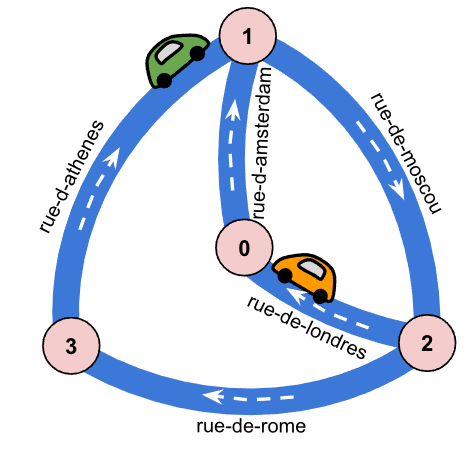
\includegraphics[width=\linewidth]{img/hashcode/figure5.png}
    % 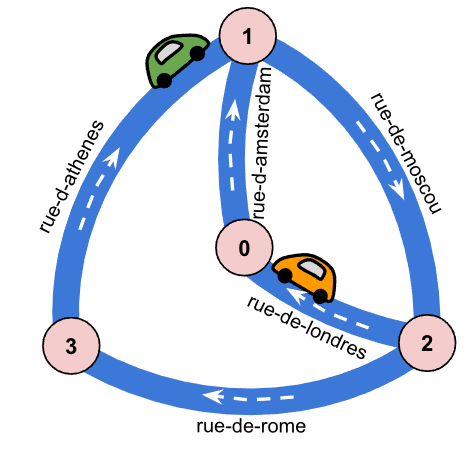
\includegraphics[width=.6\linewidth]{img/hashcode/figure5.png}
    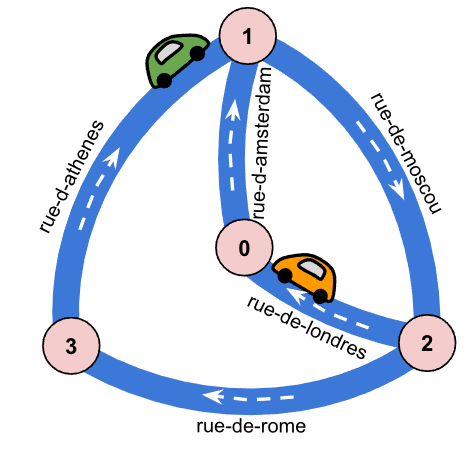
\includegraphics[width=.5\linewidth]{img/hashcode/figure5.png}
    \caption[Visualization of dataset A]{
        Visualization of dataset A \cite{google2023google}.
    }
    \label{fig:hashcode_dataset_a}
\end{figure}

\paragraph{A - An example: 4 parameters} Simple toy problem dataset used for debugging (see Figure~\ref{fig:hashcode_dataset_a}).

\paragraph{B - By the ocean: 5,974 parameters} Dataset based on a real city plan of Lisbon, Portugal (see Figure~\ref{fig:hashcode_dataset_b}).

\begin{figure}[h]
    \centering
    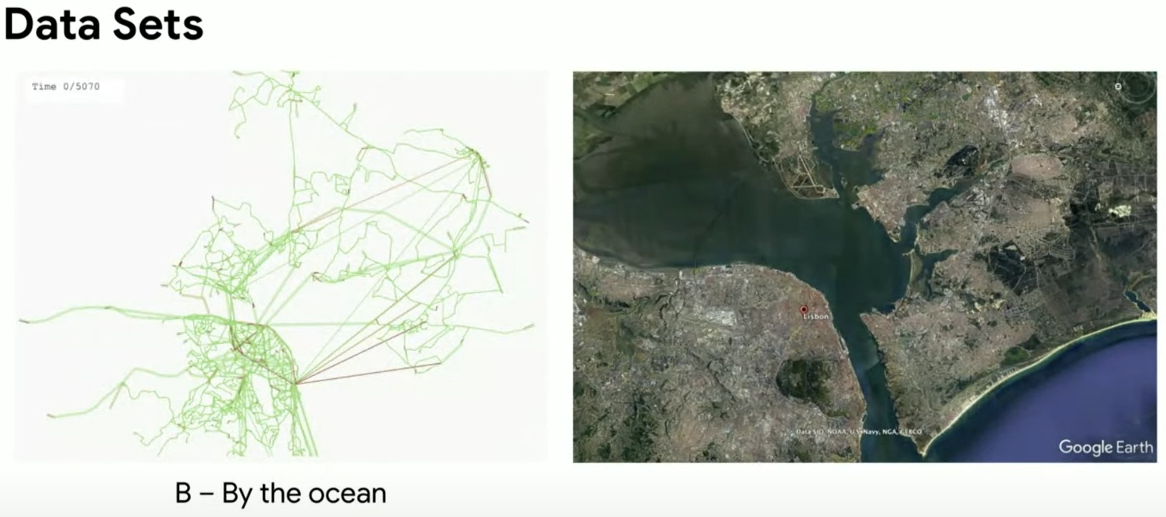
\includegraphics[width=\linewidth]{img/screenshots/hashcode_datasets_b.png}
    % 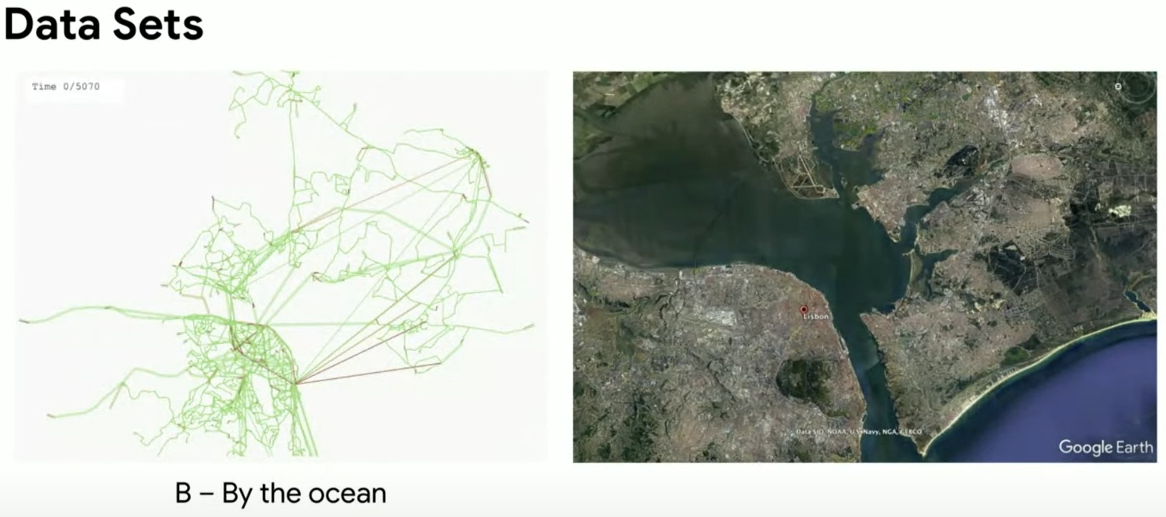
\includegraphics[width=.8\linewidth]{img/screenshots/hashcode_datasets_b.png}
    \caption[Visualization of dataset B]{
        Dataset B based on the real data of Lisbon on the right. Screenshot from \href{https://www.youtube.com/watch?v=YPOVd-hQUjA}{Hash Code 2021: Online Qualification Round Livestream}.
    }
    \label{fig:hashcode_dataset_b}
\end{figure}

\paragraph{C - Checkmate: 14,008 parameters} Dataset with a chessboard-like pattern and regular structure of intersections and streets (see Figure~\ref{fig:hashcode_dataset_c_e}).

% https://codeforces.com/blog/entry/88188#comment-765574
\paragraph{D - Daily commute: 167,748 parameters} By far the largest dataset with a challenging-to-navigate network from the \textit{Barabási-Albert} distribution \cite{albert2002statistical}.

\paragraph{E - Etoile: 1,386 parameters} Nicknamed \textit{Etoile}\footnote{\textit{Étoile} means star in French.}, this dataset is a one big star, meaning there is one very important intersection in the middle with hundrets of incoming streets (see Figure~\ref{fig:hashcode_dataset_c_e}).

\paragraph{F - Forever jammed: 10,002 parameters} Medium sized dataset but again with a complex network difficult to optimize.

\begin{figure}[h]
    \centering
    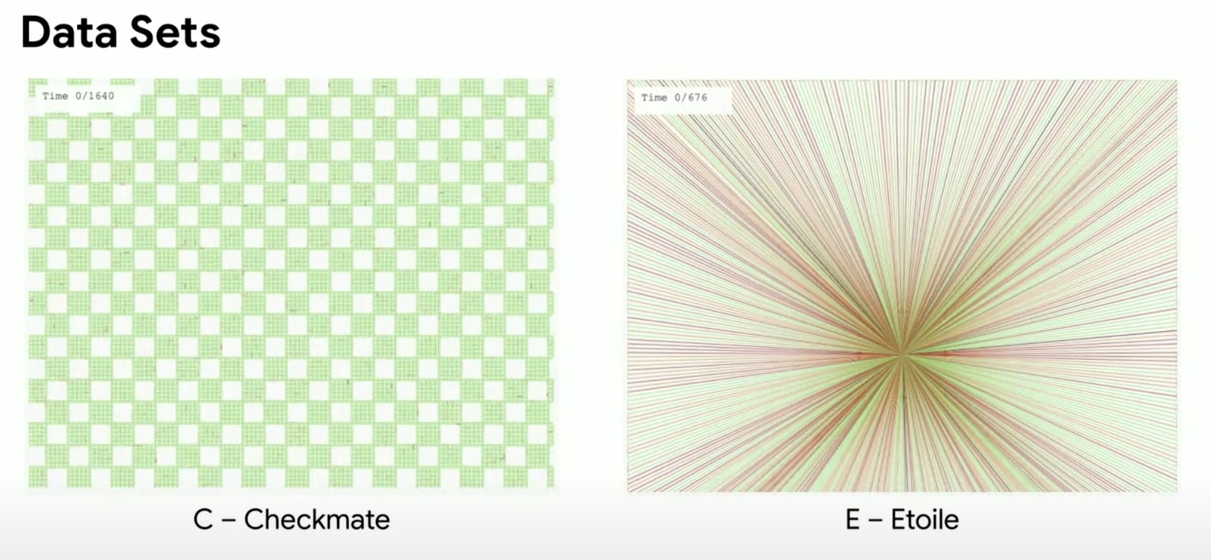
\includegraphics[width=\linewidth]{img/screenshots/hashcode_datasets_c_e.png}
    % 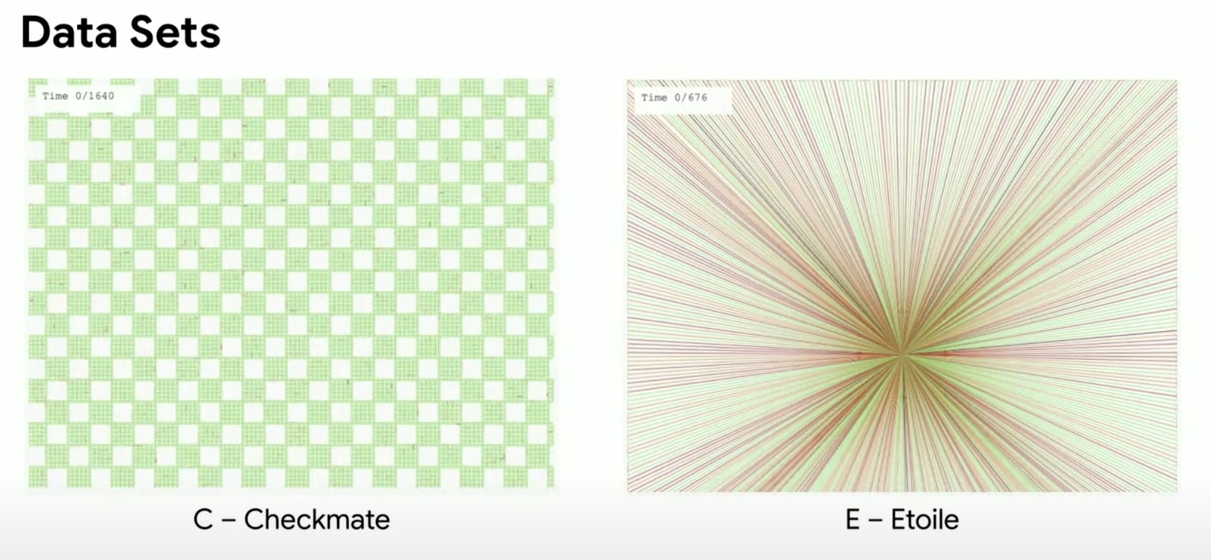
\includegraphics[width=.8\linewidth]{img/screenshots/hashcode_datasets_c_e.png}
    \caption[Visualization of datasets C and E]{
        Visualization of datasets C and E. Screenshot from \href{https://www.youtube.com/watch?v=YPOVd-hQUjA}{Hash Code 2021: Online Qualification Round Livestream}.
    }
    \label{fig:hashcode_dataset_c_e}
    \end{figure}

\subsection{Score normalization} \label{subsec:score_normalization}

As mentioned in Section~\ref{sec:competition_overview}, each dataset yields an absolute score within a different range. To compare the performance across all datasets, we normalize the scores to a 0--1 scale, where 0 represents our baseline solution (see Section~\ref{sec:initial_schedules} for details), and 1 corresponds to the maximum known score\footnote{See the maximum known scores at \\\url{https://github.com/sagishporer/hashcode-2021-qualification\#score}.} for the dataset. Note that the baseline is already a good solution, so there may be limited room for improvement---for example, in dataset B.

\section{Simulator} \label{sec:simulator}

This section provides a brief overview of the custom simulator that we developed to serve as a black-box fitness function for the optimization algorithms. We discuss the motivation behind its design and describe the functionality relevant to the optimization process.
For further information on using the simulator or regarding its implementation, please refer to the User guide in Appendix~\ref{chap:user_guide} and the Developer documentation in Appendix~\ref{chap:developer_documentation}.

\medskip

Our simulator replaces the original competition evaluation system, which was accessible only through the competition website via a user interface and is no longer available. It also adds several features on top of the original system.
The simulator is written in C++ to be as fast and efficient as possible, and is wrapped as a Python package using the powerful pybind11 library~\cite{jakob2017pybind11}, making it very convenient to use.
Inspired by libraries such as NumPy\footnote{\url{https://numpy.org/}} and PyTorch\footnote{\url{https://pytorch.org/}}, our goal is to provide an easy-to-use interface and seamless integration with the vital Python ecosystem, without compromising on top-tier performance.

Following are the features of the simulator package that are important for optimization. These features are implemented in C++ and exposed through a lightweight Python API:
\begin{itemize}
    \item Reading and storing the input data.
    \item Creating initial schedules using several different options listed in Section~\ref{sec:initial_schedules}.
    \item Running the simulation to evaluate given schedules.
    \item Retrieving and updating schedules in a format described in Section~\ref{subsec:schedules_format}.
\end{itemize}

The only case where larger data are passed between C++ and Python is when retrieving and updating the schedules.
Since the optimization loop is implemented in Python using parts of the DEAP library~\cite{fortin2012deap}, it must retrieve the schedules from the simulator, modify them externally, and then send them back into the simulator to evaluate their score.

\chapter{Theoretical background of used optimization methods}

\section{Local search}

\subsection{Hill climbing}

\subsection{Simulated annealing}

\section{Genetic algorithm}

\chapter{Theory of optimization methods} \label{chap:optimization_methods}

In this chapter, we cover the theory of the methods we use to optimize the Traffic signaling problem. Specifically, we describe \textit{hill climbing} (Section~\ref{sec:hill_climbing}), \textit{simulated annealing} (Section~\ref{sec:simulated_annealing}) and \textit{genetic algorithm} (Section~\ref{sec:genetic_algorithm}). In Section~\ref{sec:initialization} and Section~\ref{sec:parallelization} we discuss common methods for initializing and parallelizing the algorithms.

In optimization, the goal is to find the best state according to an objective function, also known as a \textit{fitness function}. In other words, the fitness function is a problem-specific function that defines how well a solution solves a particular problem.
Because the state space of optimized problems can be very large or even infinite, systematic search methods are often unsuitable. Instead, we can use the so-called \textit{heuristic algorithms}. These algorithms do not guarantee to find the~best solution but are frequently used in practice because they can find good solutions in reasonable time. Our three chosen methods are all examples of heuristic algorithms.

\section{Hill climbing} \label{sec:hill_climbing}

Hill climbing \cite{russell2020artificial, luke2013essentials} is one of the simplest local search algorithms. It keeps track of the current state and on each iteration moves to the neighboring state with the highest value, i.e., it moves in the direction that provides the biggest improvement. If there are no neighboring states with a higher value, the algorithm terminates. The greedy nature of hill climbing is both its strength and its weakness. It can make rapid progress towards a good solution but once it gets stuck in a local optimum it cannot escape it.

A lot of variants of this algorithm exist. In our experiments, we use a version called \textit{first-choice hill climbing} (see Algorithm~\ref{alg:first_choice_hill_climbing}). This version randomly generates next states until it finds one with a higher value than the current state and then moves to this state. This strategy works well when there are many neighboring states or when no defined neighborhood structure exists, which is exactly our case.

\begin{algorithm}
% https://tex.stackexchange.com/questions/150184/how-to-avoid-uppercase-function-name-while-using-function
%\algrenewcommand\textproc{} % disable uppercase function name

\begin{algorithmic}
\caption{First-choice hill climbing} \label{alg:first_choice_hill_climbing}
\Function{First-Choice-Hill-Climbing}{$problem$}
\State $current \gets problem$.I\textsc{nitial}
\For{$t = 1$ \textbf{to} M\textsc{ax\_iterations}}
    \State $next \gets$ a randomly generated next state
    \If{$\Call{Value}{next} > \Call{Value}{current}$}
        \State $current \gets next$
    \EndIf
\EndFor
\State \Return $current$
\EndFunction
\end{algorithmic}
\end{algorithm}

\section{Simulated annealing} \label{sec:simulated_annealing}

Simulated annealing \cite{russell2020artificial, luke2013essentials} builds up on the idea of hill climbing and solves the problem of getting stuck in local optima (see Algorithm~\ref{alg:simulated_annealing}). In each iteration, it randomly generates a next state. If the state is better, it is always accepted. Otherwise, the worse state is accepted with some probability. The probability decreases exponentially with how much worse the state is and with the current value of the ``cooling'' schedule. By allowing moves to worse states, the algorithm can escape local optima and therefore find better solutions.

The idea of the cooling schedule is inspired by the process of annealing in metallurgy, where metals are heated to a high temperature and then slowly cooled down to reach a strong, crystalline structure. Analogously, we want to allow worse moves more often at the beginning during the exploration phase and then gradually decrease that chance to hopefully converge to the best solution. Obviously, the choice of the schedule is absolutely crucial for the performance of the algorithm and has to be tuned specifically for each problem.

\begin{algorithm}
    % https://tex.stackexchange.com/questions/150184/how-to-avoid-uppercase-function-name-while-using-function
    %\algrenewcommand\textproc{} % disable uppercase function name
    
    \begin{algorithmic}
    \caption{Simulated annealing} \label{alg:simulated_annealing}
    \Function{Simulated-Annealing}{$problem$, $schedule$}
    \State $current \gets problem$.I\textsc{nitial}
    \For{$t = 1$ \textbf{to} M\textsc{ax\_iterations}}
        \State $T \gets$ \Call{$schedule$}{$t$}
        \State $next \gets$ a randomly generated next state
        \State $\Delta E \gets \Call{Value}{next} - \Call{Value}{current}$
        \If{$\Delta E > 0$}
            \State $current \gets next$
        \Else
            \State $current \gets next$ with probability $e^{\Delta E / T}$
        \EndIf
    \EndFor
    \State \Return $current$
    \EndFunction
    \end{algorithmic}
\end{algorithm}

\section{Genetic algorithm} \label{sec:genetic_algorithm}

% https://martinpilat.com/en/nature-inspired-algorithms/evolutionary-algorithms-introduction
% https://martinpilat.com/en/nature-inspired-algorithms/evolutionary-algorithms-continuous-and-combinatorial-optimization

Initially proposed by Holland \cite{holland1975adaptation} and Goldberg \cite{goldberg1989genetic}, genetic algorithm \cite{russell2020artificial,vanneschi2023lectures} belongs to the group of \textit{evolutionary algorithms}. Those algorithms are inpired by the seminal Darwin's theory of evolution, particularly by the idea of \textit{natural selection} \cite{darwin1859origin}. It states that the individuals with better traits suited to their environment are more likely to adapt, survive and reproduce. Over successive generations, these advantageous traits become more common in the population, leading to the emergence of new species.

This biological motivation is translated into the context of evolutionary algorithms in the following way. We work with a set of individuals called a \textit{population}. Each individual in this population represents a solution to a given problem. The algorithm runs in iterations called \textit{generations}. In each generation, it selects some individuals, modifies them using the so-called \textit{genetic operators} and then selects which individuals survive to the next generation. The selection process prefers individuals that are better at solving the problem, i.e., individuals with higher fitness.
There are many different evolutionary algorithms with even more variations that follow the previous description. Let us now focus specifically on the genetic algorithm (see Algorithm~\ref{alg:genetic_algorithm}).

\begin{algorithm}
    % https://tex.stackexchange.com/questions/150184/how-to-avoid-uppercase-function-name-while-using-function
    %\algrenewcommand\textproc{} % disable uppercase function name
    
    \begin{algorithmic}
    \caption{Genetic algorithm} \label{alg:genetic_algorithm}
    \Function{Genetic-Algorithm}{$population$}
    \State $population \gets \Call{Initialize}{population}$
    \For{$t = 1$ \textbf{to} M\textsc{ax\_iterations}}
    \State $population \gets \Call{Evaluate}{population}$
    \State $selected \gets \Call{Select}{population}$
    % Bad formatting of ff in math mode
    % https://tex.stackexchange.com/questions/6046/bad-formating-of-ff-in-math-mode
    \State $\mathit{offspring} \gets \Call{Reproduce}{selected}$
    \State $population \gets \mathit{offspring}$
    \EndFor
    \State \Return $population$
    \EndFunction
    \\
    \Function{Reproduce}{$selected$}
    \State $\mathit{offspring} \gets$ empty list
    \For{$parent1$, $parent2$ \textbf{in} $selected$}
    \State $child1$, $child2 \gets$ \Call{Crossover}{$parent1$, $parent2$}
    % algorithmic: one line if
    % https://tex.stackexchange.com/questions/624457/algorithmic-put-if-else-and-endif-into-the-same-line
    % \State\algorithmicif\ small probability \algorithmicthen\ $child1 \gets \Call{Mutate}{child1}$
    % \State\algorithmicif\ small random probability \algorithmicthen\ $child2 \gets \Call{Mutate}{child2}$
    \If{small random probability}
    \State $child1 \gets \Call{Mutation}{child1}$
    \EndIf
    \If{small random probability}
    \State $child2 \gets \Call{Mutation}{child2}$
    \EndIf
    \State add $child1$, $child2$ to $\mathit{offspring}$
    \EndFor
    \State \Return $\mathit{offspring}$
    \EndFunction
\end{algorithmic}
\end{algorithm}

\subsection{Selection}

For the selection of parents for the next generation, common methods include the \textit{roulette wheel selection} and the \textit{tournament selection} \cite{vanneschi2023lectures}. Roulette wheel selection selects individuals with a probability directly proportional to their fitness. Its downside is that it does not work for negative fitness and can be sensitive to changes in fitness values. Tournament selection works by repeatedly sampling a few individuals and selecting the best one among them. Thus, it is not dependent on specific values and can be used with any fitness function.

\subsection{Crossover and mutation}

The offspring is created from the selected parents using genetic operators \textit{crossover} and \textit{mutation}. Crossover combines two parents to produce two new children. There are many different ways to perform crossover, the most common being the \textit{one-point crossover}. Since individuals are usually represented as strings or arrays of numbers, one-point crossover simply picks a point in the individual and creates two new individuals by copying the first part from one parent and the second part from the other parent and vice versa. This can be extended to the \textit{two-point crossover} or the \textit{k-point crossover} in general. Other examples of crossover, e.g., if an individual represents a permutation and simple swapping of parts cannot be used, include the \textit{order crossover (OX)} or the \textit{partially mapped crossover (PMX)} \cite{vanneschi2023lectures}, also known as the \textit{partially matched crossover (PMX)}.

Mutation is a small random change in an individual. It is used to introduce variability into the population and to prevent the algorithm from getting stuck in local optima. Mutation is usually more problem-specific than crossover and is often customized to the problem at hand. Some common examples are the \textit{bit-flip mutation} for binary strings, the \textit{uniform} and the \textit{gaussian} mutations, i.e., a mutation replacing a value with a number drawn from one of these distributions, or the \textit{index shuffle} mutation for permutations.

\bigskip

The created offspring directly replaces the old population and the process repeats. Unfortunately, this mechanism does not guarantee that the best individual will be preserved in the next generation. To prevent this, a technique called \textit{elitism} can be used. Elitism always transfers a few of the best parents to the next generation, ensuring that the best solution found so far is not lost. The rest of the population is then filled with the offspring as previously mentioned.

\section{Initialization} \label{sec:initialization}

In all of the previously mentioned algorithms, we start with some initial state or population of initial states. The simplest and most straightforward way is to generate the initial state randomly. This is often good enough, but if the state space is large or the problem is complex, the algorithm can be very inefficient. Instead, we can try to come up with some smarter heuristic method to start in a more promising region of the search space. This is especially beneficial if we have some prior knowledge about the problem because we can help the algorithm skip exploring irrelevant parts of the search space, effectively reducing the number of iterations needed to find a good solution. An example of such a heuristic initialization is the \textit{nearest neighbors} initialization for the \textit{Traveling Salesman Problem (TSP)}, where the next node in the sequence is chosen as the closest unvisited node instead of generating the sequence randomly.

However, using heuristics for initialization can be a double-edged sword as it can lead to \textit{premature convergence} \cite{vanneschi2023lectures}. This means losing the diversity of solutions too early and getting stuck in a local optimum.
When using optimization algorithms, it is always important to balance the trade-off between \textit{exploration} and \textit{exploitation} \cite{luke2013essentials}. Exploration is a process of searching the search space for new solutions, while exploitation is a process of refining the current solutions.

\section{Parallelization} \label{sec:parallelization}

As hinted in the previous sections, heuristic algorithms can run for a long time. It is not uncommon to compute hundreds of thousands of fitness evaluations---imagine a genetic algorithm with a population size of 200, run for 1000 generations. These evaluations can take a while, especially if they are simulations, games, neural network training, or similar. As a result, we may want to use parallelization to speed up this process and fully utilize our computational resources.

Single-state methods like hill climbing and simulated annealing are inherently sequential and thus difficult to parallelize. But we can at least run multiple independent instances of the algorithm in parallel. Note that this is different from methods like \textit{beam search}, where useful information is shared between the instances.

For population methods like genetic algorithm, parallelization makes much more sense. The most common way is to run the fitness evaluations of individuals in parallel. This is great because the evaluations are completely independent of each other and the fitness computation is often the biggest bottleneck of the whole algorithm. Other parts, such as mutation and crossover, can also be parallelized across individuals, but these are usually much faster than the evaluation and may not provide much speedup, if any.

\chapter{Practical description of the optimization algorithms}

\section{Section 1}

\section{Section 2}

\chapter{Experiments} \label{chap:experiments}

In this chapter, we explain the setup of our experiments, describe how we measure the performance of different methods, and present the results. All experiments were performed using either the AMD EPYC 9454 or the AMD EPYC 9474F CPUs.

\section{Datasets}

Here we briefly describe all datasets provided with the Google Hash Code Traffic signaling problem. This is important because the datasets have different sizes and structures.

\paragraph{A - An example: 4 parameters} Simple toy problem dataset used for debugging (See Figure~\ref{fig:hashcode_dataset_a}).

\paragraph{B - By the ocean: 5,974 parameters} Dataset based on a real city plan of Lisbon, Portugal (See Figure~\ref{fig:hashcode_dataset_b}).

\paragraph{C - Checkmate: 14,008 parameters} Dataset with a chessboard-like pattern and regular structure of intersections and streets (See Figure~\ref{fig:hashcode_dataset_c_e}).

% https://codeforces.com/blog/entry/88188#comment-765574
\paragraph{D - Daily commute: 167,748 parameters} By far the largest dataset with a challenging-to-navigate network from the \textit{Barabási-Albert} distribution.

\paragraph{E - Etoile: 1,386 parameters} Nicknamed \textit{Etoile}\footnote{\textit{Étoile} means star in French.}, this dataset is a one big star, meaning there is one very important intersection in the middle with hundrets of incoming streets (See Figure~\ref{fig:hashcode_dataset_c_e}).

\paragraph{F - Forever jammed: 10,002 parameters} Medium sized dataset but again with a complex network difficult to optimize.

\begin{figure}
    \centering
    % 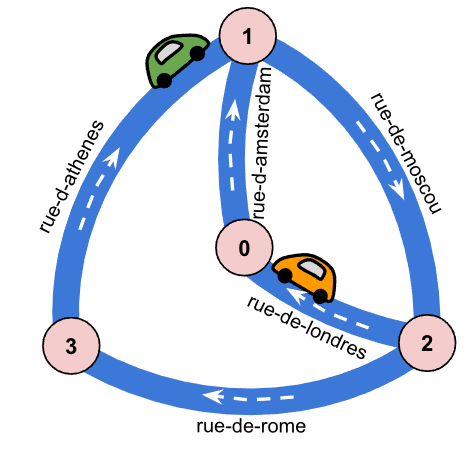
\includegraphics[width=\linewidth]{img/hashcode/figure5.png}
    % 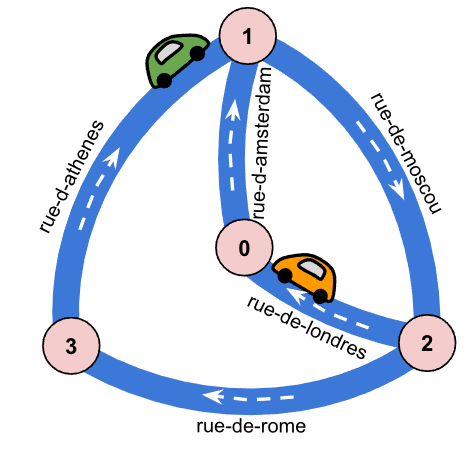
\includegraphics[width=.6\linewidth]{img/hashcode/figure5.png}
    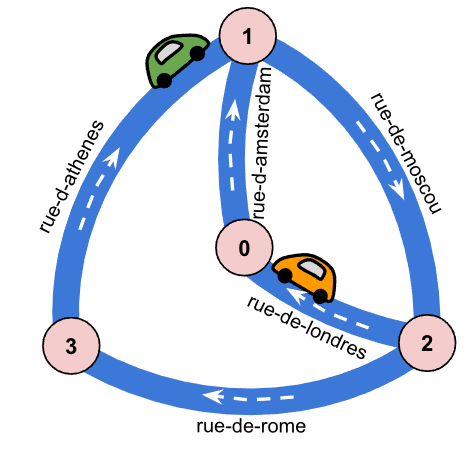
\includegraphics[width=.5\linewidth]{img/hashcode/figure5.png}
    \caption[Visualization of dataset A]{
        Visualization of dataset A \cite{google2023google}.
    }
    \label{fig:hashcode_dataset_a}
\end{figure}

\begin{figure}
    \centering
    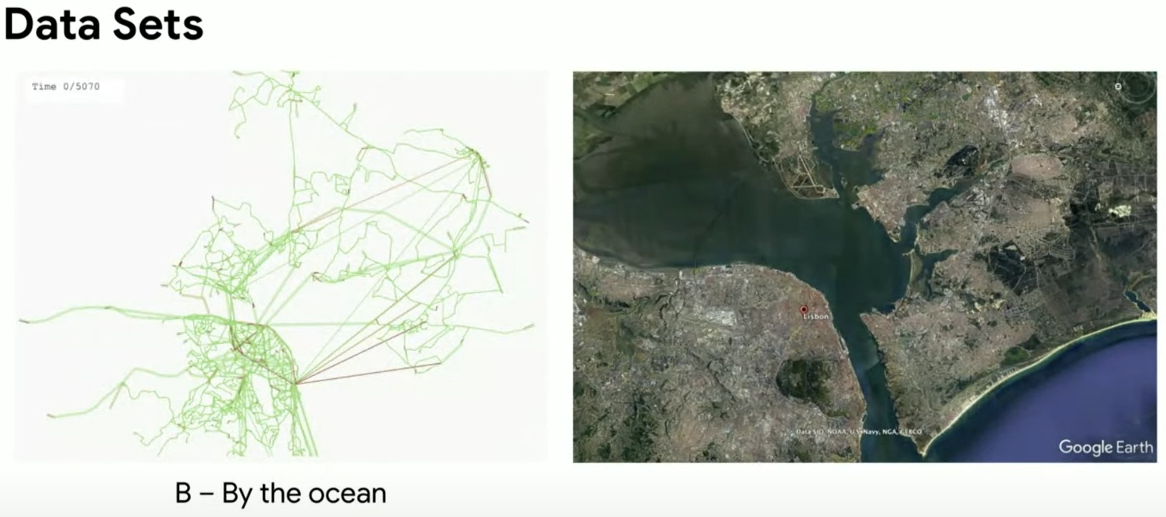
\includegraphics[width=\linewidth]{img/screenshots/hashcode_datasets_b.png}
    % 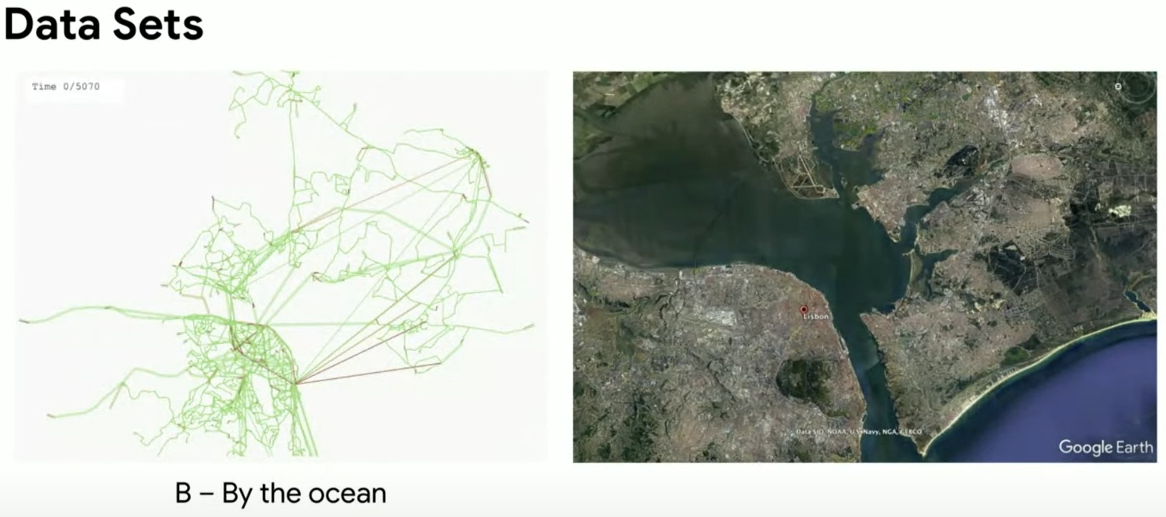
\includegraphics[width=.8\linewidth]{img/screenshots/hashcode_datasets_b.png}
    \caption[Visualization of dataset B]{
        Dataset B based on the real data of Lisbon on the right\footnotemark.
    }
    \label{fig:hashcode_dataset_b}
\end{figure}

\footnotetext{Screenshot from \href{https://www.youtube.com/watch?v=YPOVd-hQUjA}{Hash Code 2021: Online Qualification Round Livestream}.}

\begin{figure}
    \centering
    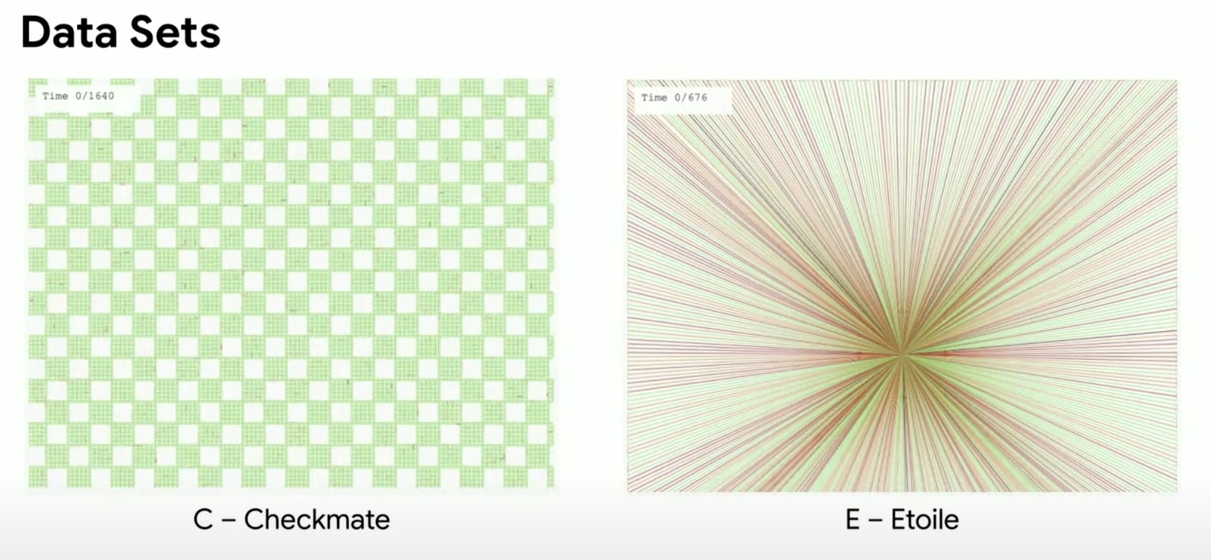
\includegraphics[width=\linewidth]{img/screenshots/hashcode_datasets_c_e.png}
    % 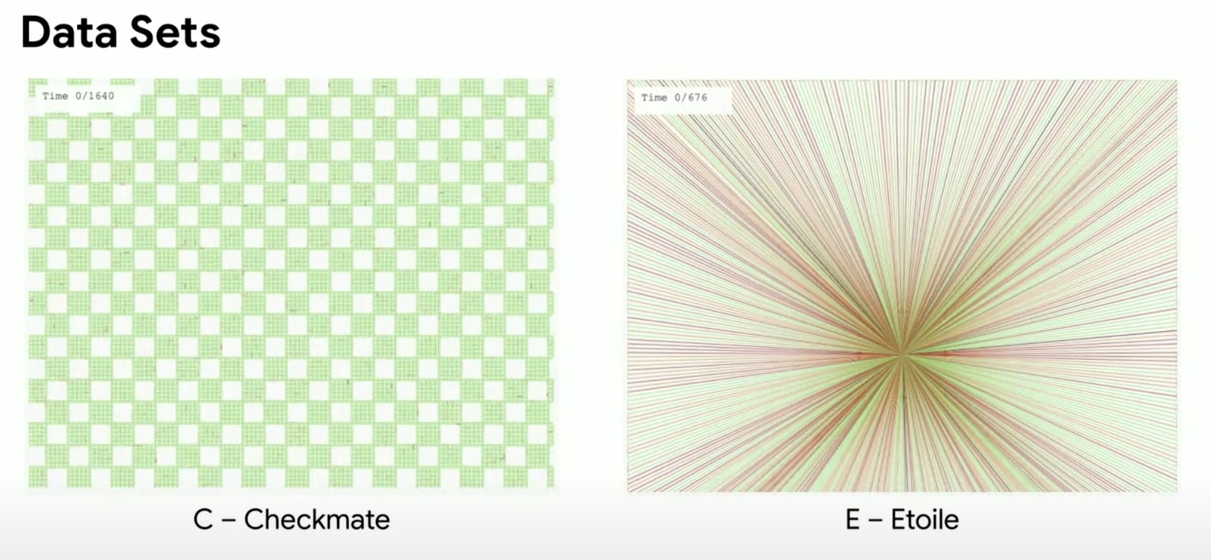
\includegraphics[width=.8\linewidth]{img/screenshots/hashcode_datasets_c_e.png}
    \caption[Visualization of datasets C and E]{
        Datasets C and E\footnotemark.
        }
        \label{fig:hashcode_dataset_c_e}
    \end{figure}
    
\footnotetext{See previous footnote.}

\bigskip

As previously stated, each dataset yields an absolute score in different range. To compare the performance across all datasets, we normalize the scores to a 0--1 range. 0 is a baseline solution with default order and default times and 1 is the maximum known score for the dataset. Note that the baseline is already a good solution and there may not be much room to improve further, e.g., in dataset B.

\section{Experiment 1: Initialization}

In the first experiment, we compare the performance of different initialization methods across all datasets. The goal is to figure out how much we can improve the baseline solution by using a ``smarter'' initialization and which initialization methods to use for further optimization.

\subsection*{Methodology}

We compare three initialization methods: \textit{adaptive}---adaptive order and default times, \textit{random}---random order and default times, and \textit{scaled}---default order and scaled times. Since the random method is stochastic, it was run 100 times and averaged. The rest of the methods are deterministic and therefore run only once.

\begin{figure}
    \centering
    % 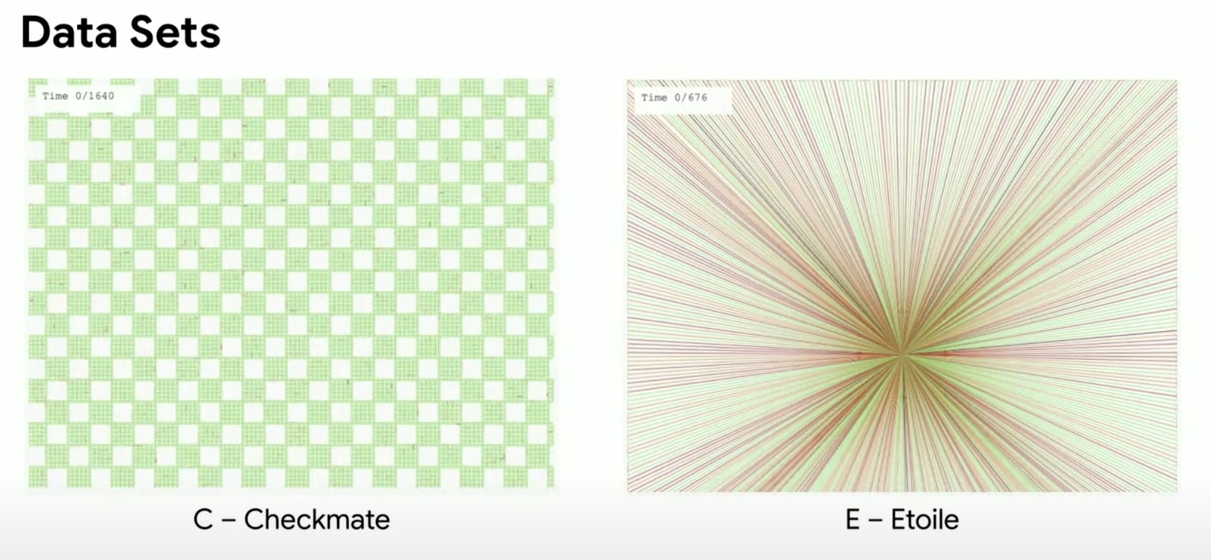
\includegraphics[width=\linewidth]{img/screenshots/hashcode_datasets_c_e.png}
    % 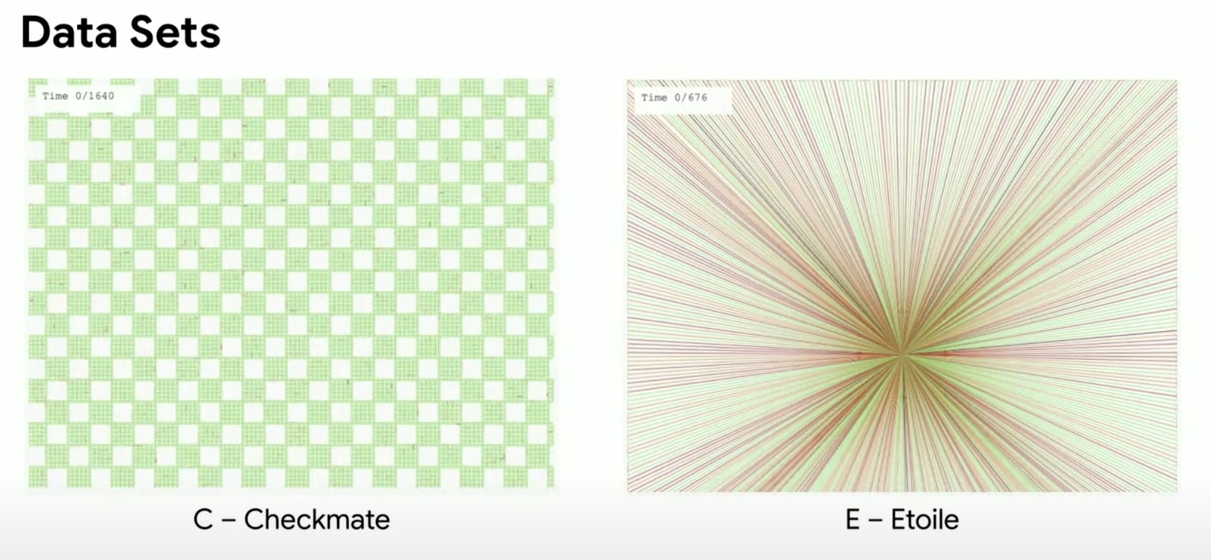
\includegraphics[width=.8\linewidth]{img/screenshots/hashcode_datasets_c_e.png}
    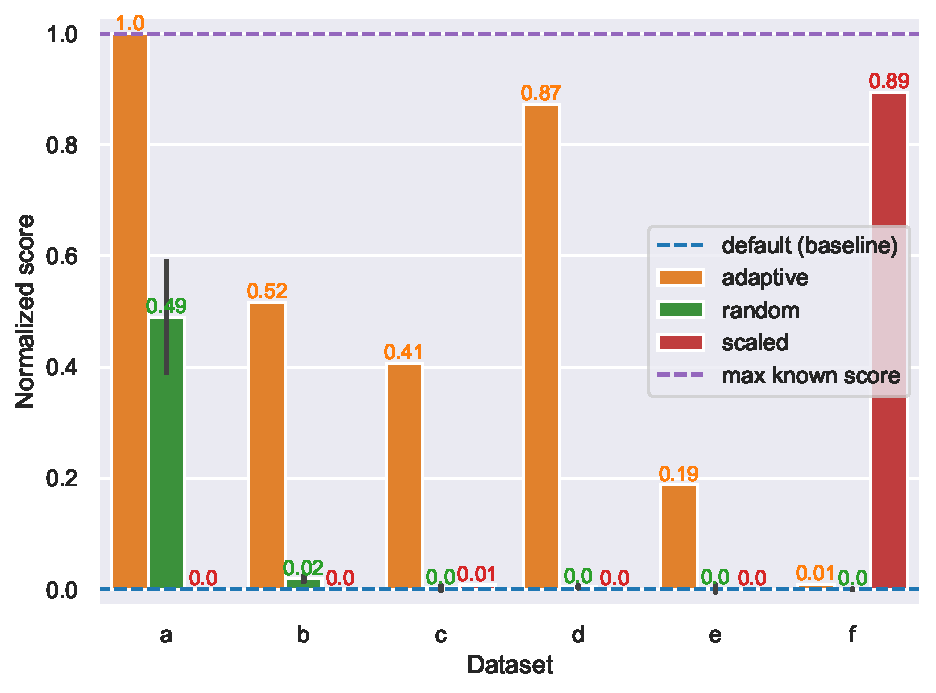
\includegraphics[width=\linewidth]{img/experiments/init_experiment.pdf}
    \caption[Initialization Experiment]{
        Initialization Experiment
    }
    \label{fig:init_experiment}
\end{figure}

\subsection*{Results}

The results are shown in Figure~\ref{fig:init_experiment}. Overall, the adaptive method provides the biggest improvement over the baseline. It also yields a really high score for the largest dataset D. The only exception is the dataset F, where the otherwise mediocre scaled method performs really well. The random method generally performs the same as the baseline but it can still be a good initialization starting point if we care about variety and randomness in the solution. 

\section{Experiment 2: Optimization}

In the second experiment, we compare different optimization methods on datasets B--F. The goal is to find if some method is superior to others or if the ideal method is dataset-dependent. We also want to see how much we can improve from the starting solutions.

\subsection*{Methodology}

We compare the three previously mentioned optimization methods: \textit{genetic algorithm}, \textit{hill climbing} and \textit{simulated annealing}. For each dataset and method, 10 runs with different seeds were performed and averaged to obtain reliable results. ...

\subsection*{Results}

\begin{figure}
    \centering
    % 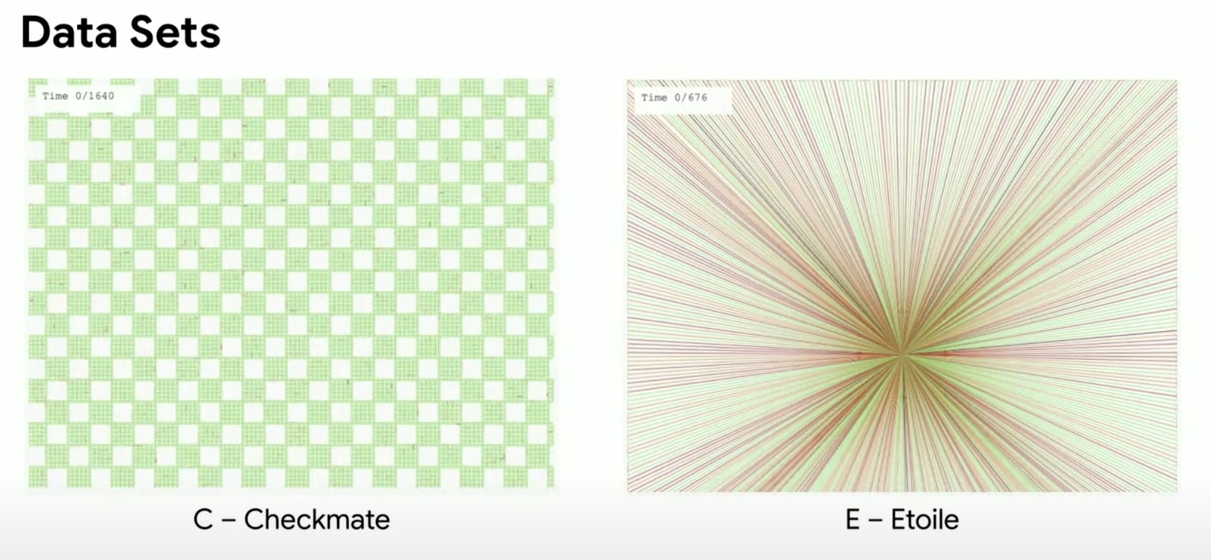
\includegraphics[width=\linewidth]{img/screenshots/hashcode_datasets_c_e.png}
    % 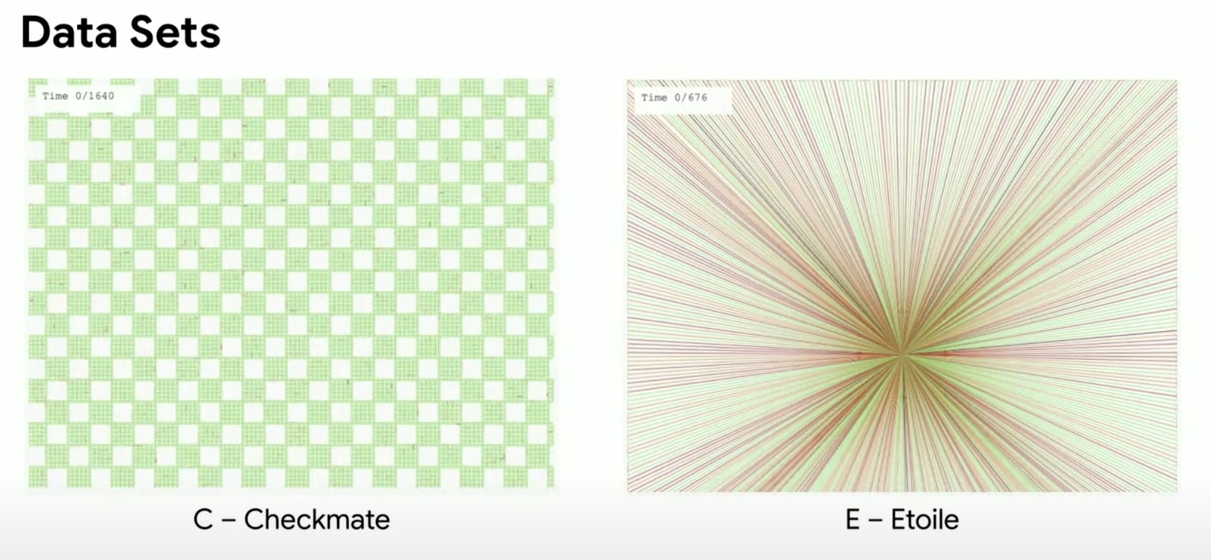
\includegraphics[width=.8\linewidth]{img/screenshots/hashcode_datasets_c_e.png}
    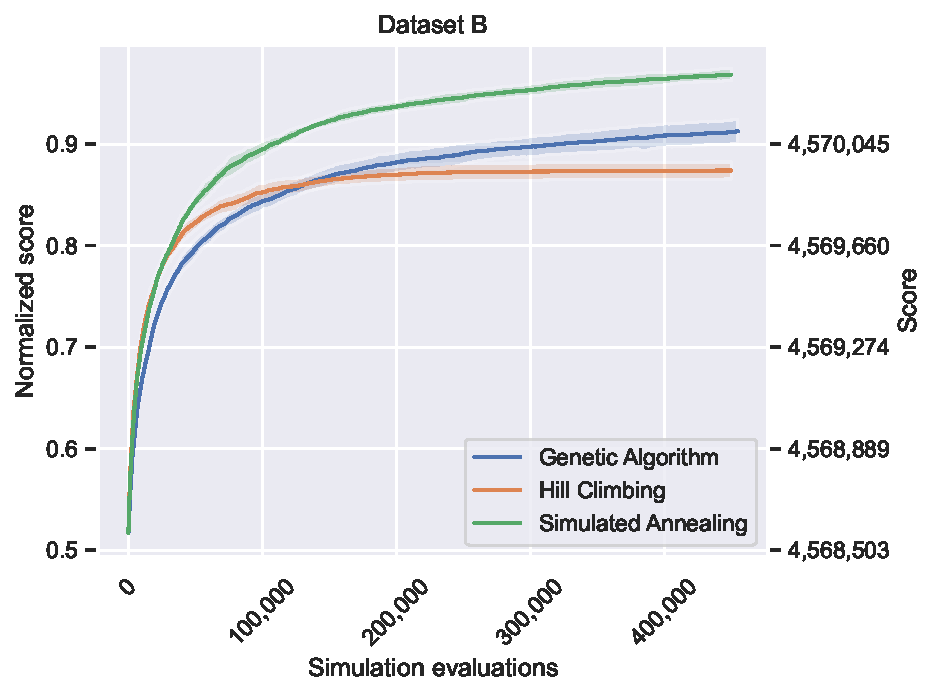
\includegraphics[width=\linewidth]{img/experiments/b_Genetic Algorithm_Hill Climbing_Simulated Annealing.pdf}
    \caption[Dataset B Experiment]{
        Dataset B Experiment
    }
    \label{fig:dataset_b_experiment}
\end{figure}

\begin{figure}
    \centering
    % 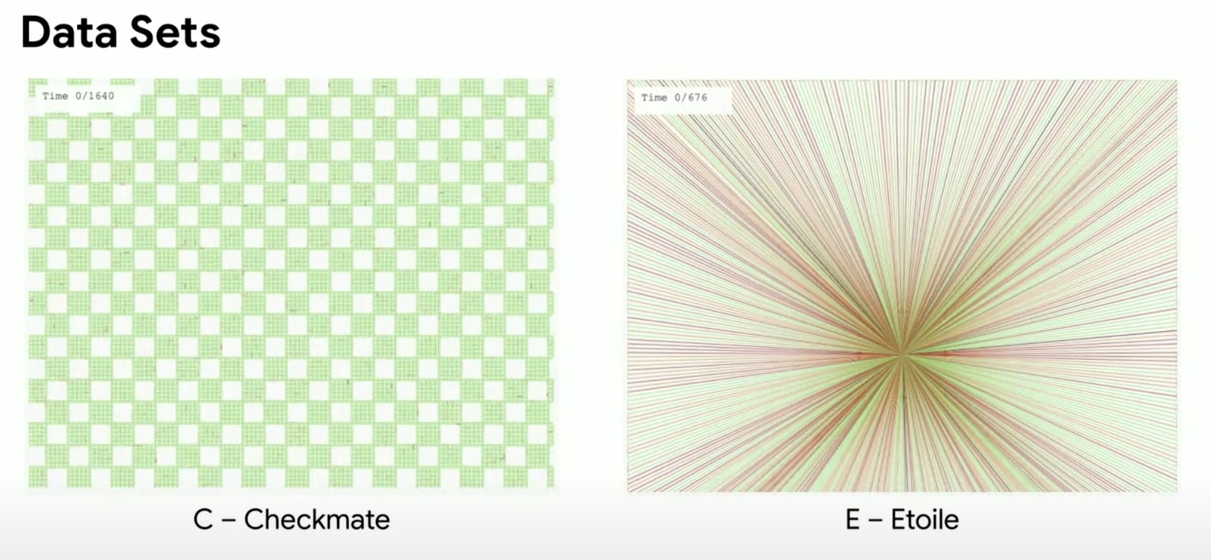
\includegraphics[width=\linewidth]{img/screenshots/hashcode_datasets_c_e.png}
    % 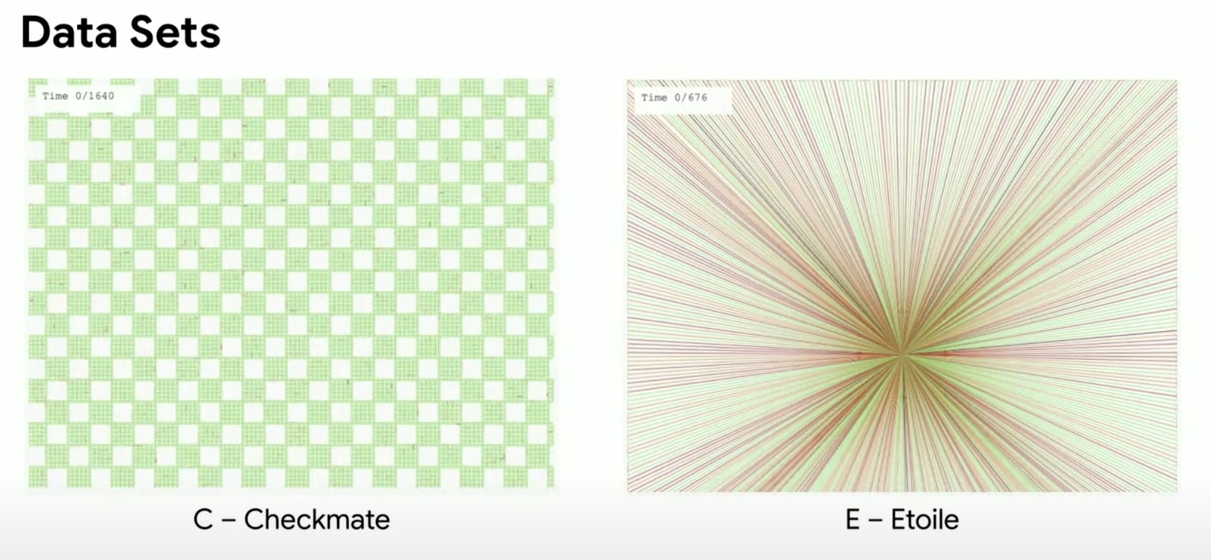
\includegraphics[width=.8\linewidth]{img/screenshots/hashcode_datasets_c_e.png}
    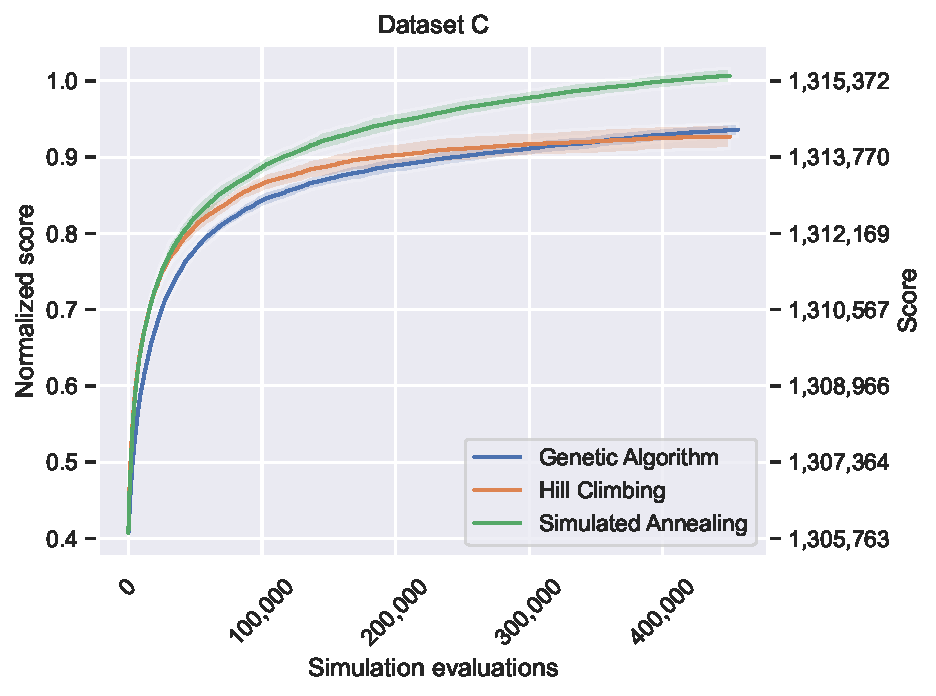
\includegraphics[width=\linewidth]{img/experiments/c_Genetic Algorithm_Hill Climbing_Simulated Annealing.pdf}
    \caption[Dataset C Experiment]{
        Dataset C Experiment
    }
    \label{fig:dataset_c_experiment}
\end{figure}

\begin{figure}
    \centering
    % 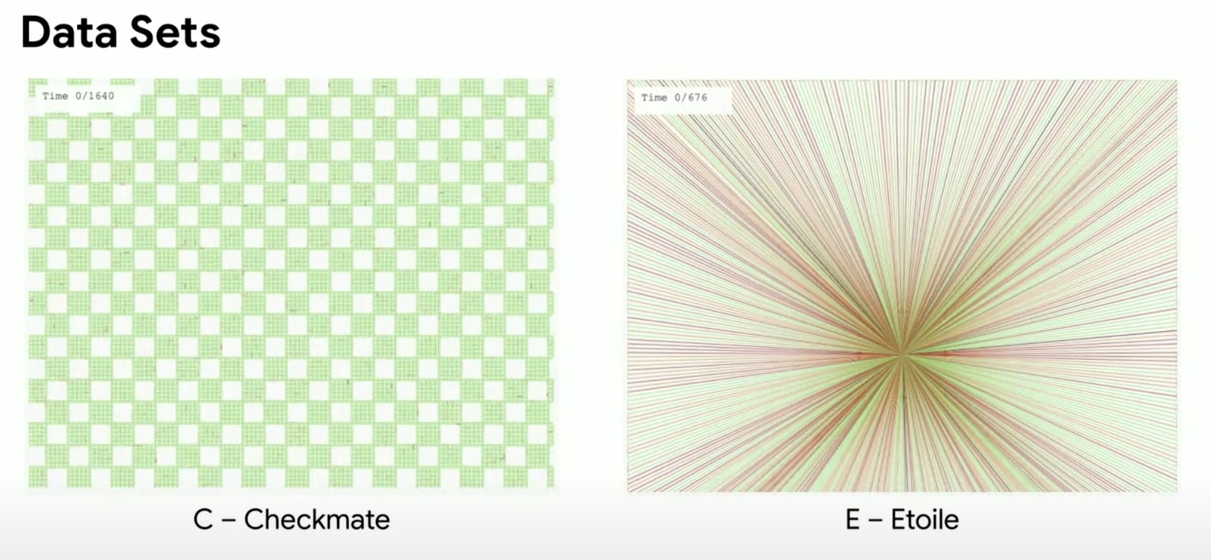
\includegraphics[width=\linewidth]{img/screenshots/hashcode_datasets_c_e.png}
    % 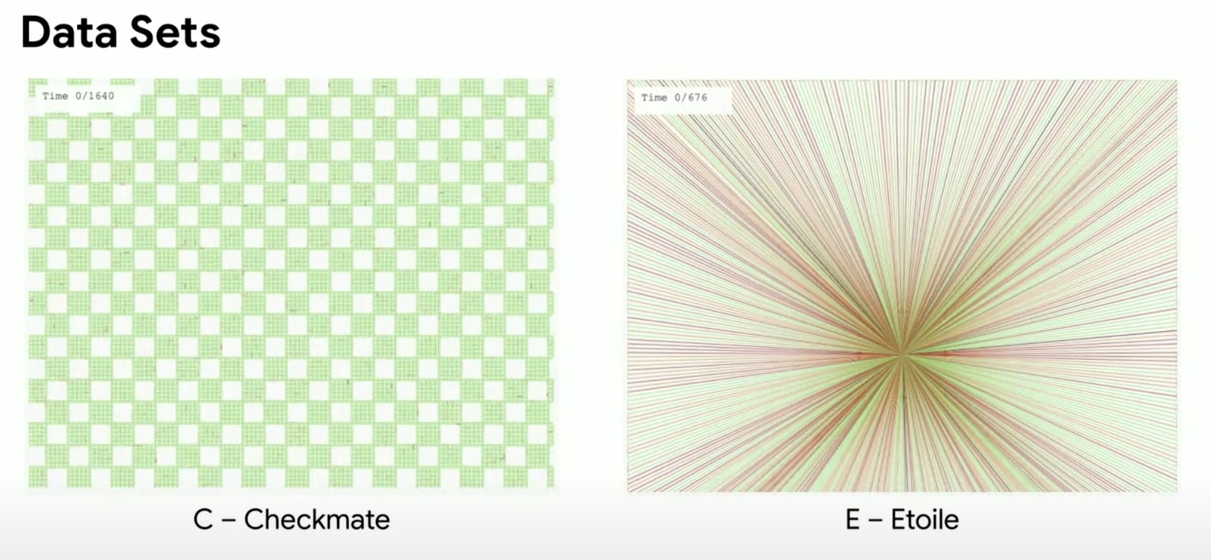
\includegraphics[width=.8\linewidth]{img/screenshots/hashcode_datasets_c_e.png}
    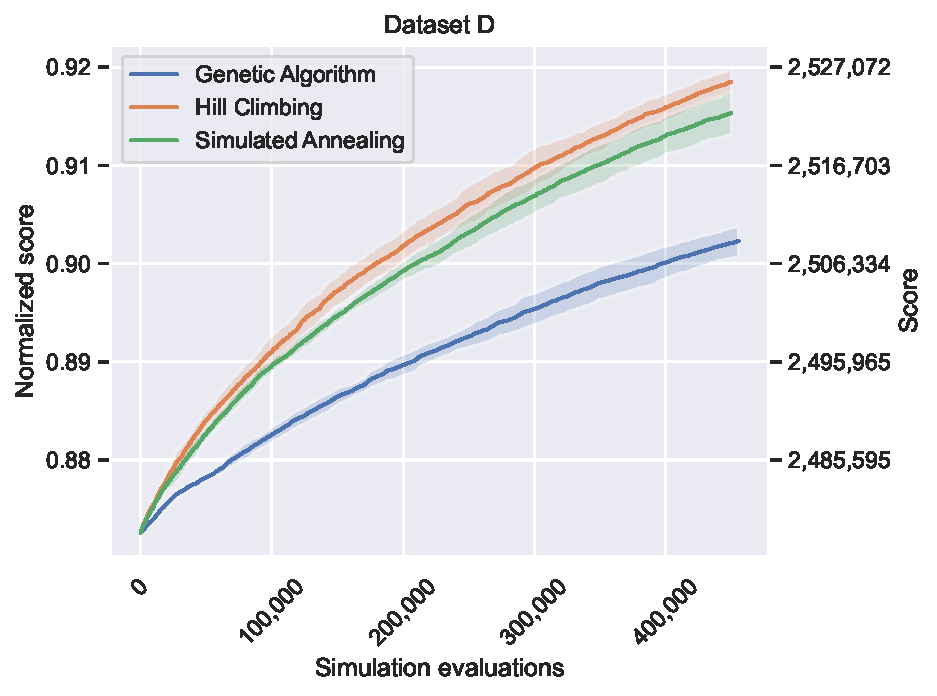
\includegraphics[width=\linewidth]{img/experiments/d_Genetic Algorithm_Hill Climbing_Simulated Annealing.pdf}
    \caption[Dataset D Experiment]{
        Dataset D Experiment
    }
    \label{fig:dataset_d_experiment}
\end{figure}

\begin{figure}
    \centering
    % 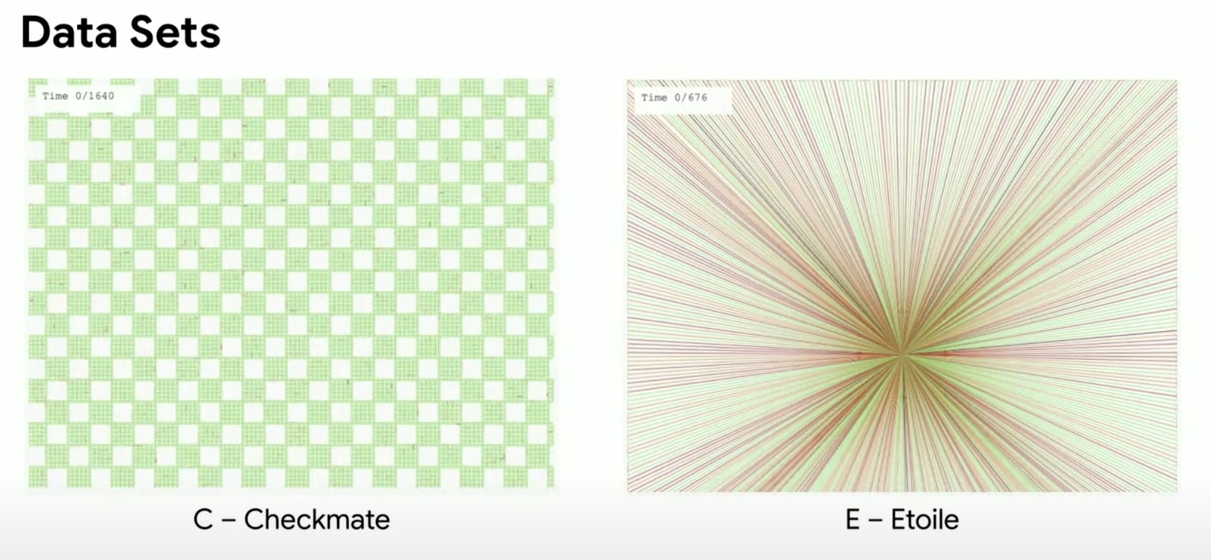
\includegraphics[width=\linewidth]{img/screenshots/hashcode_datasets_c_e.png}
    % 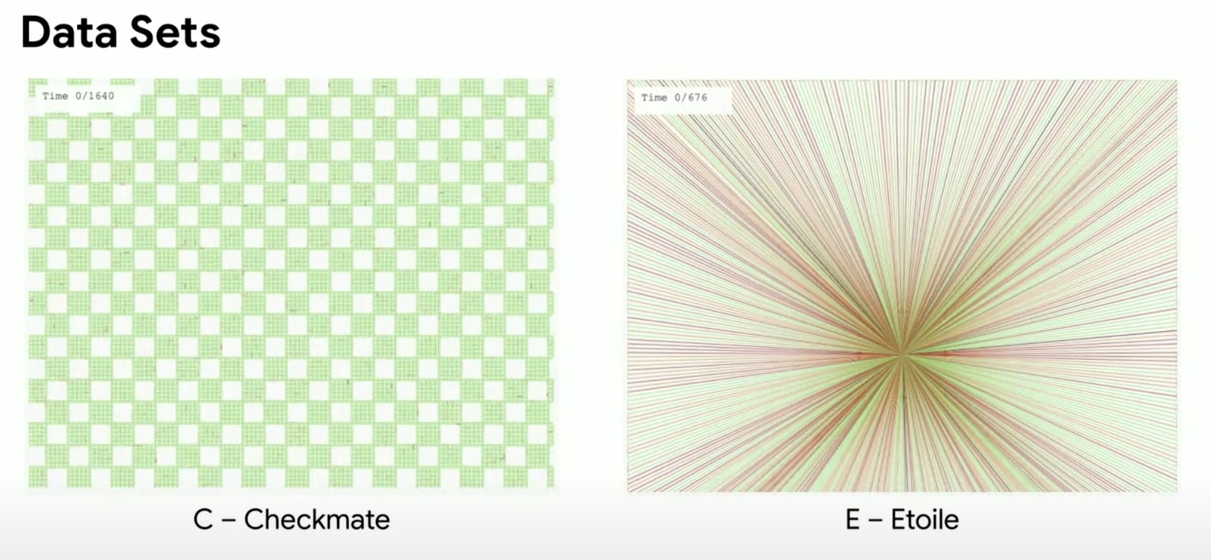
\includegraphics[width=.8\linewidth]{img/screenshots/hashcode_datasets_c_e.png}
    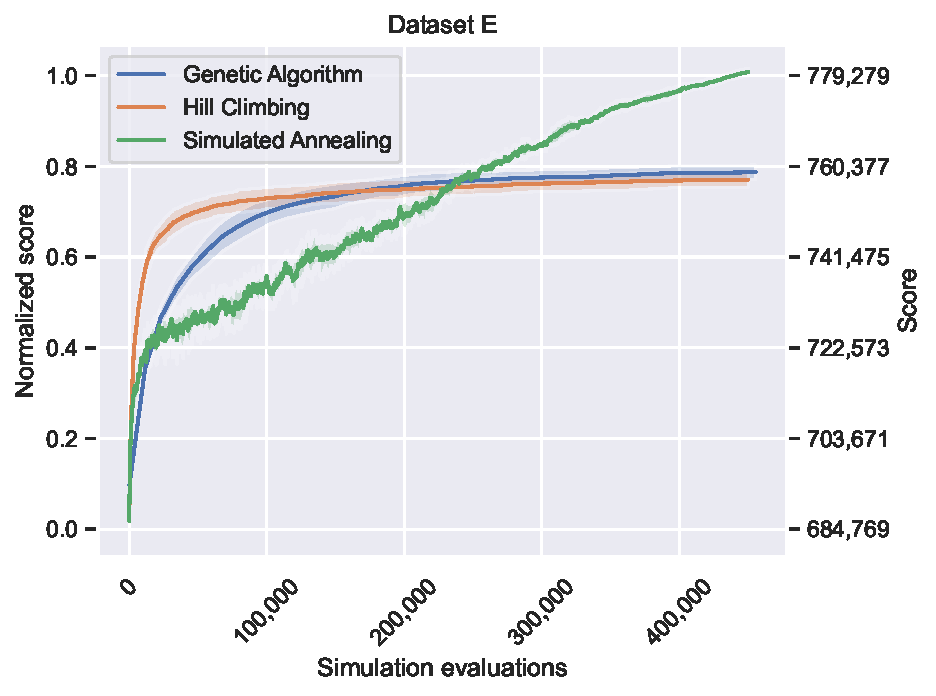
\includegraphics[width=\linewidth]{img/experiments/e_Genetic Algorithm_Hill Climbing_Simulated Annealing.pdf}
    \caption[Dataset E Experiment]{
        Dataset E Experiment
    }
    \label{fig:dataset_e_experiment}
\end{figure}

\begin{figure}
    \centering
    % 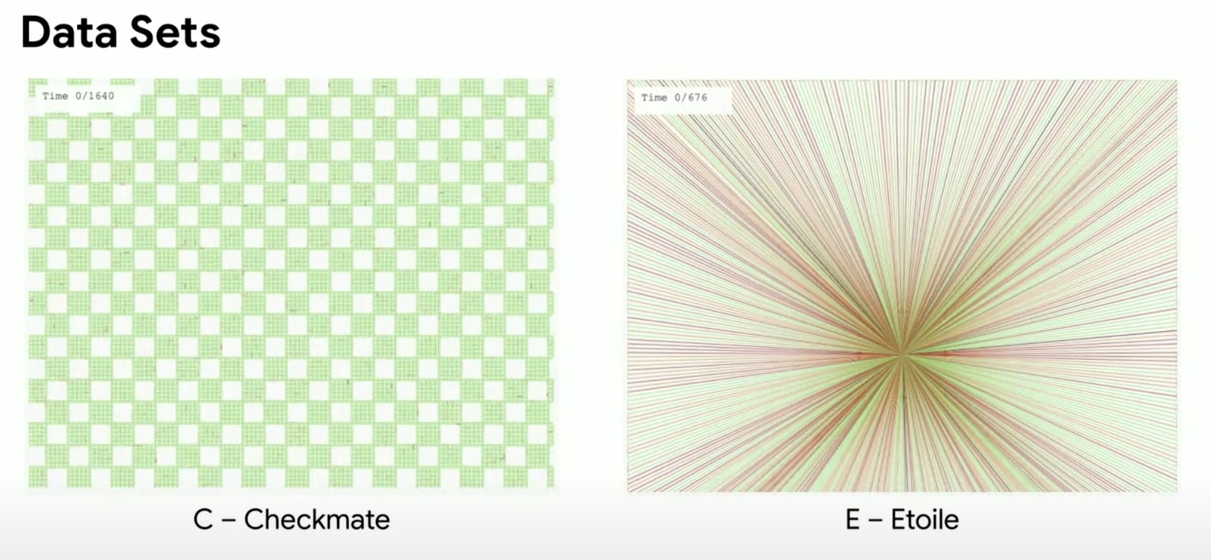
\includegraphics[width=\linewidth]{img/screenshots/hashcode_datasets_c_e.png}
    % 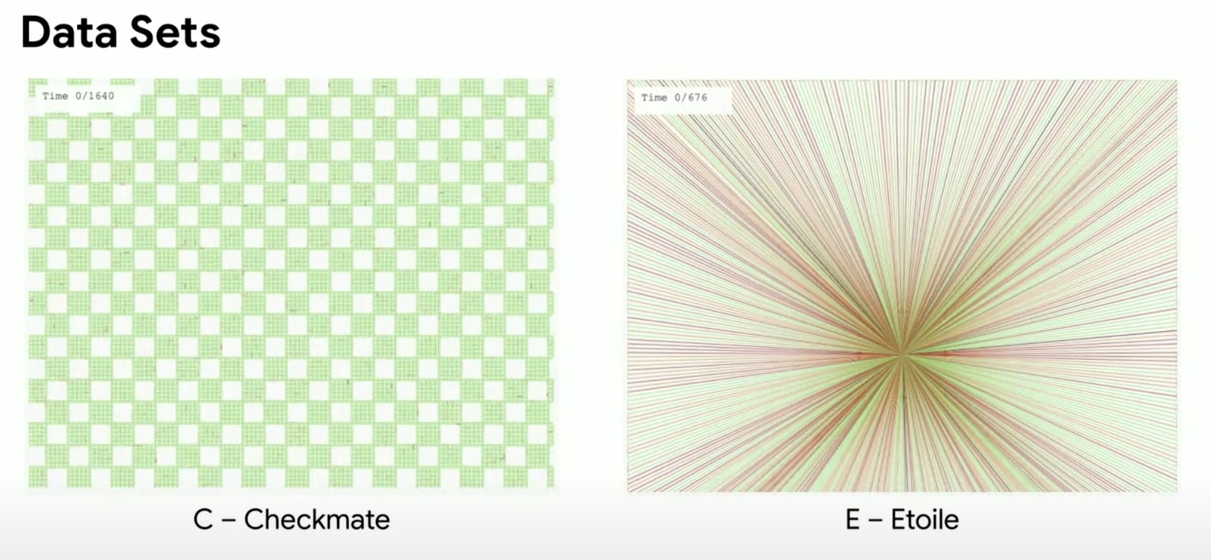
\includegraphics[width=.8\linewidth]{img/screenshots/hashcode_datasets_c_e.png}
    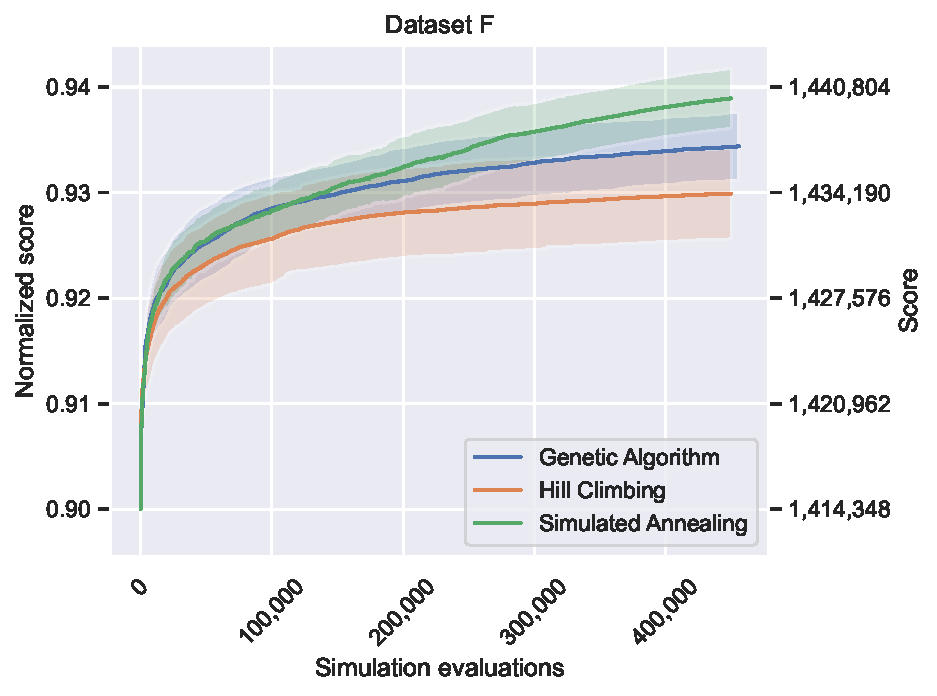
\includegraphics[width=\linewidth]{img/experiments/f_Genetic Algorithm_Hill Climbing_Simulated Annealing.pdf}
    \caption[Dataset F Experiment]{
        Dataset F Experiment
    }
    \label{fig:dataset_f_experiment}
\end{figure}

% \begin{table}[b!]

% \centering
% %% Tabulka používá následující balíčky:
% %%   - booktabs (\toprule, \midrule, \bottomrule)
% %%   - dcolumn (typ sloupce D: vycentrovaná čísla zarovnaná na
% %%     desetinnou čárku
% %%     Všimněte si, že ve zdrojovém kódu jsou desetinné tečky, ale
% %%     tisknou se čárky.
% %% Dále používáme příkazy \pulrad a \mc definované v makra.tex

% \begin{tabular}{l@{\hspace{1.5cm}}D{.}{,}{3.2}D{.}{,}{1.2}D{.}{,}{2.3}}
% \toprule
%  & \mc{} & \mc{\textbf{Směrod.}} & \mc{} \\
% \pulrad{\textbf{Efekt}} & \mc{\pulrad{\textbf{Odhad}}} & \mc{\textbf{chyba}$^a$} &
% \mc{\pulrad{\textbf{P-hodnota}}} \\
% \midrule
% Abs. člen     & -10.01 & 1.01 & \mc{---} \\
% Pohlaví (muž) & 9.89   & 5.98 & 0.098 \\
% Výška (cm)    & 0.78   & 0.12 & <0.001 \\
% \bottomrule
% \multicolumn{4}{l}{\footnotesize \textit{Pozn:}
% $^a$ Směrodatná chyba odhadu metodou Monte Carlo.}
% \end{tabular}

% \caption{Maximálně věrohodné odhady v~modelu M.}\label{tab03:Nejaka}

% \end{table}

\begin{table}
% uncomment the following line if you use the fitted top captions for tables
% (see the \floatsetup[table] comments in `macros.tex`.
%\floatbox{table}[\FBwidth]{
\centering\footnotesize\sf
\begin{tabular}{llrl}
\toprule
Column A & Column 2 & Numbers & More \\
\midrule
Asd & QWERTY & 123123 & -- \\
Asd qsd 1sd & \textcolor{red}{BAD} & 234234234 & This line should be helpful. \\
Asd & \textcolor{blue}{INTERESTING} & 123123123 & -- \\
Asd qsd 1sd & \textcolor{violet!50}{PLAIN WEIRD} & 234234234 & -- \\
Asd & QWERTY & 123123 & -- \\
\addlinespace % a nice non-intrusive separator of data groups (or final table sums)
Asd qsd 1sd & \textcolor{green!80!black}{GOOD} & 234234299 & -- \\
Asd & NUMBER & \textbf{123123} & -- \\
Asd qsd 1sd & \textcolor{orange}{DANGEROUS} & 234234234 & (no data) \\
\bottomrule
\end{tabular}
%}{  % uncomment if you use the \floatbox (as above), erase otherwise
\caption{An example table.  Table caption should clearly explain how to interpret the data in the table. Use some visual guide, such as boldface or color coding, to highlight the most important results (e.g., comparison winners).}
%}  % uncomment if you use the \floatbox
\label{tab:z}
\end{table}

\begin{table}
% uncomment the following line if you use the fitted top captions for tables
% (see the \floatsetup[table] comments in `macros.tex`.
%\floatbox{table}[\FBwidth]{
\centering\footnotesize\sf
\begin{tabular}{llrl}
\toprule
Dataset & GA & HC & SA \\
\midrule
B & \textbf{0.95} & 0.90 & 0.85 \\
C & 0.90 & 0.88 & 0.87 \\
D & 0.98 & 0.96 & 0.95 \\
E & 0.92 & 0.91 & 0.89 \\
F & 0.93 & 0.90 & 0.88 \\
\bottomrule
% Asd & QWERTY & 123123 & -- \\
% Asd qsd 1sd & \textcolor{red}{BAD} & 234234234 & This line should be helpful. \\
% Asd & \textcolor{blue}{INTERESTING} & 123123123 & -- \\
% Asd qsd 1sd & \textcolor{violet!50}{PLAIN WEIRD} & 234234234 & -- \\
% Asd & QWERTY & 123123 & -- \\
% \addlinespace % a nice non-intrusive separator of data groups (or final table sums)
% Asd qsd 1sd & \textcolor{green!80!black}{GOOD} & 234234299 & -- \\
% Asd & NUMBER & \textbf{123123} & -- \\
% Asd qsd 1sd & \textcolor{orange}{DANGEROUS} & 234234234 & (no data) \\
% \bottomrule
\end{tabular}
%}{  % uncomment if you use the \floatbox (as above), erase otherwise
\caption{An example table.  Table caption should clearly explain how to interpret the data in the table. Use some visual guide, such as boldface or color coding, to highlight the most important results (e.g., comparison winners).}
%}  % uncomment if you use the \floatbox
\label{tab:results}
\end{table}


\chapter*{Conclusion}
\addcontentsline{toc}{chapter}{Conclusion}

\section*{Future Work / Improvements}
% \addcontentsline{toc}{section}{Future Work / Improvements}


%%% Bibliography
%%% Bibliography (literature used as a source)
%%%
%%% We employ biblatex to construct the bibliography. It processes
%%% citations in the text (e.g., the \cite{...} macro) and looks up
%%% relevant entries in the bibliography.bib file.
%%%
%%% See also biblatex settings in thesis.tex.

%%% Generate the bibliography. Beware that if you cited no works,
%%% the empty list will be omitted completely.

% We let bibliography items stick out of the right margin a little
\def\bibfont{\hfuzz=2pt}

\printbibliography[heading=bibintoc]

%%% If case you prefer to write the bibliography manually (without biblatex),
%%% you can use the following. Please follow the ISO 690 standard and
%%% citation conventions of your field of research.

% \begin{thebibliography}{99}
%
% \bibitem{lamport94}
%   {\sc Lamport,} Leslie.
%   \emph{\LaTeX: A Document Preparation System}.
%   2nd edition.
%   Massachusetts: Addison Wesley, 1994.
%   ISBN 0-201-52983-1.
%
% \end{thebibliography}


%%% Figures used in the thesis (consider if this is needed)
\listoffigures

%%% Tables used in the thesis (consider if this is needed)
%%% In mathematical theses, it could be better to move the list of tables to the beginning of the thesis.
\listoftables

%%% Abbreviations used in the thesis, if any, including their explanation
%%% In mathematical theses, it could be better to move the list of abbreviations to the beginning of the thesis.
\chapwithtoc{List of Abbreviations}

\begin{description}
	\item[GA] Genetic Algorithm
	\item[HC] Hill Climbing
	\item[SA] Simulated Annealing 
\end{description}

% \printglossary[title={List of Abbreviations}]

%%% Doctoral theses must contain a list of author's publications
\ifx\ThesisType\TypePhD
\chapwithtoc{List of Publications}
\fi

%%% Attachments to the thesis, if any. Each attachment must be referred to
%%% at least once from the text of the thesis. Attachments are numbered.
%%%
%%% The printed version should preferably contain attachments, which can be
%%% read (additional tables and charts, supplementary text, examples of
%%% program output, etc.). The electronic version is more suited for attachments
%%% which will likely be used in an electronic form rather than read (program
%%% source code, data files, interactive charts, etc.). Electronic attachments
%%% should be uploaded to SIS. Allowed file formats are specified in provision
%%% of the rector no. 72/2017. Exceptions can be approved by faculty's coordinator.
\appendix
% \chapter{Attachments}

% \section{First Attachment}

\chapter{User Guide} \label{chap:user_guide}

\section{Section 1}


\chapter{Developer Documentation} \label{chap:developer_documentation}

\xxx{DEAP citation \cite{fortin2012deap}.}

\section{Section 1}

\xxx{Code example...}

\begin{lstlisting}[language=Python]
from traffic_signaling import *

# Load the city plan for a specific dataset
plan = create_city_plan(data='e')
# Create a simulation for the given city plan
sim = Simulation(plan)
# Set traffic light schedules to default values
sim.default_schedules()
# Calculate the score
score = sim.score()
# Show statistics of the simulation
sim.summary()
\end{lstlisting}

\end{document}
